%%%%%
%%
%% Chalmers University of Technology Master's Thesis Template
%%
%% Jonas Einarsson (2010)
%% Adapted from work by Joel Goop
%%
%% Uses references.bib as Bibtex source
%% Uses elsevier numerical style .bst (change in settings.tex)
%%
%% DON'T FORGET: Change PDF metadata in settings.tex !!
%%
%%%%%
\documentclass[11pt,a4paper,twoside,openright]{report}

% Packages and commands file
\usepackage[utf8]{inputenc}
\usepackage[T1]{fontenc}
\usepackage[english]{babel}
\usepackage{amsmath}
\usepackage{amssymb}
\usepackage{ae}
\usepackage{icomma}
\usepackage{units}
\usepackage{color}
\usepackage{graphicx}
\usepackage{epstopdf}
%\usepackage{subfigure}
\usepackage{bbm}
\usepackage[square, numbers, sort]{natbib}
\usepackage{multirow}
\usepackage{array}
\usepackage[font=footnotesize,format=plain,labelfont=bf,up]{caption}
\usepackage{geometry}
\usepackage{fancyhdr}
\usepackage{fncychap}
\usepackage[hyphens]{url}
\usepackage[breaklinks,pdfpagelabels=false]{hyperref}
\usepackage{lettrine}
\usepackage{eso-pic}
%\usepackage{algorithm2e}
\usepackage{nomencl}
%\usepackage[style=long,nonumberlist]{glossaries}
\usepackage{setspace}


\makenomenclature
\renewcommand{\nomname}{List of Abbreviations}
%\makeglossaries

\newcommand{\rd}{\ensuremath{\mathrm{d}}}
\newcommand{\id}{\ensuremath{\,\rd}}
\newcommand{\degC}{\ensuremath{\,\unit{^\circ C}}}

% Fancyheader shortcuts
\newcommand{\setdefaulthdr}{%
\fancyhead[L]{\slshape \rightmark}%
\fancyhead[R]{ }%
\fancyfoot[C]{\thepage}%
}
\newcommand{\setspecialhdr}{%
\fancyhead[L]{ }%
\fancyhead[R]{\slshape \leftmark}%
\fancyfoot[C]{\thepage}%
}

% My own additions
\usepackage{float}
\usepackage{url}
\usepackage{subcaption}



\newcommand{\mail}[1]{\href{mailto:#1}{\nolinkurl{#1}}}
\newcommand{\backgroundpic}[3]{%
	\put(#1,#2){
		\parbox[b][\paperheight]{\paperwidth}{%
			\centering
			\includegraphics[width=\paperwidth,height=\paperheight,keepaspectratio]{#3}
			\vfill
}}}


%\usepackage{subcaption}


% Settings (Metadata)
% References, choose bst-file
\bibliographystyle{elsart-num}

% PDF Metadata and link styles
\hypersetup{
		pdftitle={Modelling of electrokinetic flow using the lattice-Boltzmann method},%
		pdfauthor={Andreas B\"{u}lling},%
    colorlinks=true,%
    citecolor=black,%
    filecolor=black,%
    linkcolor=black,%
    urlcolor=black
}

% Dropping initial letter color
\renewcommand{\LettrineFontHook}{\color[gray]{0.5}}

% Chapter headings style (fncychap)
\makeatletter
\ChNumVar{} % sets the style for digit
\ChTitleVar{\Huge\bfseries\centering} % sets the style for title
\ChRuleWidth{4pt} % Set RW=4pt
\ChNameUpperCase % Make name uppercase
\renewcommand{\DOCH}{
\centering
{\CNoV {\fontsize{60pt}{20pt}\selectfont\thechapter} }
\vskip 40\p@}
\renewcommand{\DOTI}[1]{%
\CTV\FmTi{#1}\par\nobreak
\vskip 40\p@}
\renewcommand{\DOTIS}[1]{%
\CTV\FmTi{#1}\par\nobreak
\vskip 40\p@}
\makeatother

% Single page abstract
\renewenvironment{abstract}%
{\begin{center} \bfseries \abstractname \end{center}}%
{\vspace{2\baselineskip}}%

% Figure & Table captions
\captionsetup{margin=10pt,font=small,labelfont=bf}
\captionsetup[table]{position=top}
\setlength{\extrarowheight}{4pt}
\addtolength{\headheight}{\baselineskip}

% Fancyheader (see packagescommands.tex for default/special)
\pagestyle{fancy}
\setdefaulthdr
%\setspecialhdr

%no extra spaces between paragraphs....
% \setlength{\parskip}{\baselineskip}
\raggedbottom

% Stolen settings (unknown origin):
% Alter some LaTeX defaults for better treatment of figures:
% See p.105 of "TeX Unbound" for suggested values.
% See pp. 199-200 of Lamport's "LaTeX" book for details.
%   General parameters, for ALL pages:
\renewcommand{\topfraction}{0.9}	% max fraction of floats at top
\renewcommand{\bottomfraction}{0.8}	% max fraction of floats at bottom
%   Parameters for TEXT pages (not float pages):
\setcounter{topnumber}{2}
\setcounter{bottomnumber}{2}
\setcounter{totalnumber}{4}     % 2 may work better
\setcounter{dbltopnumber}{2}    % for 2-column pages
\renewcommand{\dbltopfraction}{0.9}	% fit big float above 2-col. text
\renewcommand{\textfraction}{0.07}	% allow minimal text w. figs
%   Parameters for FLOAT pages (not text pages):
\renewcommand{\floatpagefraction}{0.7}	% require fuller float pages
% N.B.: floatpagefraction MUST be less than topfraction !!
\renewcommand{\dblfloatpagefraction}{0.7}	% require fuller float pages

% remember to use [htp] or [htpb] for placement

%nomenclature
%\makenomenclature


%definitions
%def of various quantities

\newcommand{\J}{\ensuremath{\mathbf{J}}}
\newcommand{\C}{\ensuremath{\mathrm{c}}} 
\newcommand{\rhorm}{\ensuremath{\mathrm{\rho}}} 
\newcommand{\drm}{\ensuremath{\mathrm{d}}} 
\newcommand{\Prm}{\ensuremath{\mathrm{P}}} 
\newcommand{\ux}{\ensuremath{\mathrm{u_x}}} 
\newcommand{\uy}{\ensuremath{\mathrm{u_y}}} 
\newcommand{\Rerm}{\ensuremath{\mathrm{Re}}}
\newcommand{\Pe}{\ensuremath{\mathrm{Pe}}} 
\newcommand{\psirm}{\ensuremath{\mathrm{\psi}}} 
\newcommand{\R}{\ensuremath{\mathrm{R}}} 
\newcommand{\Gi}{\ensuremath{\mathrm{G_i}}} 
\newcommand{\cnil}{\ensuremath{\mathrm{c_0}}} 
\newcommand{\lnil}{\ensuremath{\mathrm{\ell_0}}} 
\newcommand{\Vnil}{\ensuremath{\mathrm{V_0}}} 
\newcommand{\unil}{\ensuremath{\mathrm{u_0}}} 
\newcommand{\nx}{\ensuremath{\mathrm{N_x}}} 
\newcommand{\ny}{\ensuremath{\mathrm{N_y}}} 
\newcommand{\QQ}{\ensuremath{\mathrm{Q}}}

\newcommand{\ubf}{\ensuremath{\mathbf{u}}}
\newcommand{\ubar}{\ensuremath{\mathbf{\bar{u}}}}
\newcommand{\x}{\ensuremath{\mathbf{x}}}
\newcommand{\n}{\ensuremath{\mathbf{n}}}
\newcommand{\Q}{\ensuremath{\mathbf{Q}}}
\newcommand{\F}{\ensuremath{\mathbf{F}}}
\newcommand{\E}{\ensuremath{\mathbf{E}}}
\newcommand{\jj}{\ensuremath{\mathbf{j}}}
\newcommand{\cbf}{\ensuremath{\mathbf{c}}}
\newcommand{\ci}{\ensuremath{\mathbf{c}_i}}
\newcommand{\p}{\ensuremath{\mathbf{p}}}

\newcommand{\feq}{\ensuremath{f_i^{(eq)}}}
\newcommand{\feqe}[1]{\ensuremath{f_i^{(eq, #1)}}}
\newcommand{\fii}{\ensuremath{f_i}}
\newcommand{\fie}[1]{\ensuremath{f_i^{(#1)}}}
\newcommand{\rhoe}[1]{\ensuremath{\rho^{(#1)}}}
\newcommand{\Rexp}[1]{\ensuremath{\mathrm{\R}^{(#1)}}}
\newcommand{\Gie}[1]{\ensuremath{\mathrm{G_i}^{(#1)}}}
\newcommand{\je}[1]{\ensuremath{\mathbf{j}^{(#1)}}}
\newcommand{\ubare}[1]{\ensuremath{\mathbf{\bar{u}}^{(#1)}}}
\newcommand{\ue}[1]{\ensuremath{\mathbf{u}^{(#1)}}}
\newcommand{\ep}{\ensuremath{\epsilon}}
\newcommand{\pd}{\ensuremath{\ci\cdot\nabla}}
\newcommand{\bigO}[1]{\ensuremath{\mathcal{O}(#1)}}
\newcommand{\parti}[1]{\ensuremath{\partial_{#1}}}
\newcommand{\cc}[1]{\ensuremath{c_{i#1}}}
\newcommand{\uc}[1]{\ensuremath{u_{#1}^{(1)}}}
\newcommand{\dd}[2]{\ensuremath{\delta_{#1#2}}}
\newcommand{\deltasec}{\ensuremath{\dd{\alpha}{\beta}\dd{\gamma}{\delta}+
    \dd{\alpha}{\gamma}\dd{\beta}{\delta}
    +\dd{\alpha}{\delta}\dd{\beta}{\gamma}}}
\newcommand{\dab}{\ensuremath{\dd{\alpha}{\beta}}}


\newcommand{\todo}[1]{
\begin{center}\textcolor{red}{ \bf{TODO: #1}}\end{center}}



\begin{document}

% Title page and abstract
% Chalmers title page
\begin{titlepage}

\mbox{}
\vspace{50mm}
%draft text
%\begin{center} 
%\textcolor{red}{
%\framebox[1.1\width]{
%\Huge{DRAFT}
%\huge{\today}
%}
%}
%\end{center}

\AddToShipoutPicture{\backgroundpic{-4}{56.7}{include/frontpage}}
\mbox{}
\vfill
\addtolength{\voffset}{2cm}
\begin{flushleft}
	{\noindent {\huge Modelling of electrokinetic flow using the
            lattice-Boltzmann method} \\[0.3cm] \emph{\Large Thesis
            for the degree of Master of Science} \\[.8cm]
	
	{\LARGE ANDREAS B\"{U}LLING}\\[.8cm]
	
	{\Large Department of Mathematical Sciences \\
         \emph{Division of Mathematics} \\
	\textsc{Chalmers University of Technology} \\
	Gothenburg, Sweden 2012 \\
	} 
	}
\end{flushleft}

\end{titlepage}
\ClearShipoutPicture
% End Chalmers title page

\pagestyle{empty}
\newpage
\clearpage
\mbox{}

%titlepage
\newpage
\clearpage
\thispagestyle{empty}
\newgeometry{bottom=0.1cm}

\mbox{}
\vspace{45pt}

\begin{center}
\LARGE \textbf{Modelling of electrokinetic flow\\ using the
  lattice-Boltzmann method} \normalsize

\vspace{8pt}
\emph{Thesis for the degree of Master of Science}\\
\vspace{10pt}
\line(1,0){100}\\
\vspace{16pt}
\large ANDREAS B\"{U}LLING
\end{center}
\vspace{365pt}

\begin{center}
\large Department of Mathematical Sciences \\
         \emph{Division of Mathematics} \\
	\textsc{Chalmers University of Technology} \\
	Gothenburg, Sweden 2012 \\
\end{center}


\newpage
\clearpage
\thispagestyle{empty}


\mbox{}
\vspace{75pt}

\noindent Modelling of electrokinetic flow using the lattice-Boltzmann
method\\
\emph{Thesis for the degree of Master of Science}\\
ANDREAS B\"{U}LLING\\

\noindent\copyright $\;$ANDREAS B\"{U}LLING, 2012\\

\noindent Department of Mathematical Sciences \\
         \emph{Division of Mathematics} \\
	Chalmers University of Technology \\
	SE-412 96 Gothenburg\\
 Sweden\\
Telephone +46 (0)31-772 1000

\vspace{370pt}

\noindent Chalmers Reproservice\\
Gothenburg, Sweden 2012

\restoregeometry

%abstract
\newpage
\clearpage
\thispagestyle{empty}

\noindent Modelling of electrokinetic flow using the lattice-Boltzmann
method\\ 
\emph{Thesis for the degree of Master of Science}\\ 
ANDREAS B\"{U}LLING\\
Department of Mathematical Sciences \\
\emph{Division of Mathematics} \\
\textsc{Chalmers University of Technology} 

\vspace{20pt}

\begin{abstract}
The lattice-Boltzmann method is used to model flow in electrokinetic
systems. A modelling approach based on the coupling of Navier-Stokes,
Nernst-Planck and Poisson's equation of electrostatics is
utilised. Three lattice-Boltzmann methods are formulated for the three
equations respectively.

The method is implemented in \texttt{C++} with the aim of being high
performing. Topics as locality, instruction pipelines and parallel
computing are considered. The implementation is tested for a number of
classic examples with known solutions, e.g.  Taylor-Green vortex flow,
an Helmholtz equation and an advection-diffusion situation. The
computed solutions agree well with the analytic solutions.

The physical systems modelled consists mainly of various charged
channel flows of ionic solutions. Electrokinetic effects, such as
electroosmosis and the electrovicous effect are studied. This is done
in thin channels where the thickness of the electrical double layers
is comparable to the channel dimension. The electroviscous effect is
shown to slow the flow down and a local minimum is found in the
velocity profile for thick enough double layers. Other more
complicated systems are also studied; electroosmotic flow in a channel
with heterogeneously charged walls and flow in a an array of charged
squares.
\end{abstract}

\noindent \textbf{Keywords:} lattice-Boltzmann, electrokinetics,
electrohydrodynamics, Nernst-Planck, Poisson-Boltzmann,
high performance computing.

\newpage
\clearpage
\mbox{}
\newpage
\clearpage
\thispagestyle{empty}
\section*{Acknowledgements}
I would hereby like to express my gratitude to my supervisor Alexei
Heintz. You did always have time for questions and discussions even
during your spare time and on your vacation. Also the precise amount
of guidance and the freedom given is very much appreciated. I am
thankful for having been given the opportunity of working on a project
where the fields of my interest from physics, mathematics and
programming were all present.  \\[1cm]

\hfill Andreas B\"{u}lling, G\"{o}teborg, \today
\newpage
\clearpage
\mbox{}


% Table of contents
\newpage
\pagenumbering{roman}
\setcounter{page}{1}
\pagestyle{fancy}
\setspecialhdr
\tableofcontents

%List of figures
\listoffigures

%List of abbreviations    
\renewcommand*{\nompreamble}{\markboth{\uppercase{\nomname}}{\uppercase{\nomname}}}
\printnomenclature

% Main area
\newpage
\setdefaulthdr
\pagenumbering{arabic}	
\setcounter{page}{1}

% Content
\chapter{Introduction}
This thesis deals with modelling of physical problems in the
interdisciplinary field of hydrodynamics and electrostatics. The tool
used for realising this is the new and promising but somewhat immature
lattice-Boltzmann method. This is a method that is still under
development but is today used in practical applications both in
industry and academy.

\section{Background}

There is currently an ongoing project at the mathematics faculty of
Chalmers University in producing a modelling package that
should be able to deal with transport of various liquids and particles
through complicated structures. The method of choice has fallen upon
the lattice-Boltzmann method for its suitable characteristics in the
systems of interest. 

This work aims to investigate the possibility and procedure for taking
electrical effects into account in the modelling of charged
fluids. More theoretical questions about the method itself and of the
physics involved is of interest as well as how the method may be
effectively implemented on a computer.

From both industry and academy, there is a demand on the modelling of
this kind of physics. For instance, in medical sciences, accurate
modelling of transport of charged fluids is a fundamental ingredient
in understanding biological systems and to be able to manipulate
them. As a consequence of the always so present desire of more
environmental friendly ways of using the planet, automotive industry
are now engineering electrical cars. A great challenge is to produce
high performing and durable batteries, the ability to accurate
model the electrolytes in the batteries is indeed an advantage in
achieving this. 

\section{Outline}
The text is structured in five main chapters. In chapter \ref{sec:et},
the physics involved and the equations of interest are presented. This
is followed by chapter \ref{sec:lbm} where the lattice-Boltzmann
method is formulated for the different equations of interest. Also an
introduction to the method as well as some discussion on different
boundary conditions is given here. In chapter \ref{sec:hpc}, the
implementation of the method is discussed together with some general
aspects that is important to have in mind in order to produce a high
performing code. The implementation is then tested for classic
examples with known solutions in chapter \ref{sec:mb}. Finally some
results in electrokintetics are presented and discussed in chapter
\ref{sec:res}. Here, the focus is rather on the physics of the
simulated systems then on LBM aspects of the problems. These aspects,
such as grid dimensions, how LBM parameters relate to physical
quanities etc. are discussed for the problems in chapter \ref{sec:mb}.

\section{Previous work}
An extensive treatment of both theory and experiments in the field of
electrokinetics is carried out in \cite{dongquing-ren-book}. Mainly
the Poisson-Boltzmann model is used in the modelling but also in some
situations, the model used in this work based on the coupling of
Navier-Stokes, Nernst-Planck and Poisson's equation of electrostatics
is discussed. Also in \cite{ren-elvis-paper}, this modelling approach
is used. However, the computational model is not the Lattice-Boltzmann
method (LBM). 

There are a lot of formulations of the LBM for the Navier-Stokes
equations as the method typically is used in the modelling of fluid
dynamics. Not so common are formulations for the Nernst-Planck and
Poisson's equation. However there are a few, e.g. in \cite{wang-poi}
and \cite{chai_poi} formulations for the Poisson's equation is
discussed. In \cite{lbm-wang} a complete formulation for the three
equations are presented together with some example simulations of
electrokinetic systems. The formulation presented in \cite{lbm-wang}
will not be completely the same as the one used in this work as is
discussed in later chapters of this text. 


\chapter{Electrohydrodynamics in microchannels}\label{sec:et}

In this chapter, the fundamental physics behind electrokinetic flow,
important for later discussions, will be presented. Particularly, a
modelling approach based on the coupling of Navier-Stokes,
Nernst-Planck and Poission's equations is given.

\section{Basic concepts of electrokinetic flow}
Electrohydrodynamics involves the study of electric phenomena on fluid
flow. How fluids carrying electrical charges (electrolytes) react upon
external electrical fields or interact with charged objects are
examples of problems that arise in this field. 

\subsection{Electrical double layers}
As a charged object is brought into contact with an electrolyte it is,
qualitatively, easily deduced that ions with a sign of charge opposite
to that of the object will be attracted to the object and ions with
the same sign of charge will be repelled. These two distinct
categories of ions will from hereon be referred to as counter- and
co-ions respectively. In this case, for a neutral electrolyte, a
surplus of counter-ions will be present in the direct vicinity of the
object and a surplus of co-ions will be present at some other location
further from the object.
 
The area with a surplus of counter-ions in an electrolyte in contact
with a charged object is often referred to as an electrical double
layer (EDL). Two distinct regions will be formed in this area, thus
the name double layer. The two layers are often referred to as the
Stern layer (adsorbed ions) and the diffusive layer (mobile ions). The
Stern layer is usually several orders of magnitude thinner than the
diffusive layer and is therefore seldom considered when it comes to
modelling \cite{dongquing-ren-book}.  \nomenclature{EDL}{Electrical
  Double Layer}

\subsection{Electroosmosis}
As a fluid carrying a net charge, e.g. in the diffusive layer of an
EDL, is under influence of an electric field, the charged particles
will move due to the electric forces. As the charge particles move,
they will affect the surrounding liquid, causing it to move as
well. This liquid motion is often referred to as electroosmotic
flow. \cite{dongquing-ren-book}

%% Consider an electrically neutral liquid, i.e. a liquid containing the
%% same amount of positive and negative ions. When this liquid is
%% introduced to, for example, a negatively charged surface, this even
%% charge distribution is disturbed in an area close to the surface. Due
%% to the introduced electrostatic forces, positive ions will be
%% attracted to the surface leaving a positive net charge in the vicinity
%% of the surface. It is possible to divide this positively charged
%% region in the liquid into two different layers. In the direct vicinity
%% of the surface, positive ions will adsorb onto the surface making them
%% less mobile than the others in the positively net charged area closer
%% to the bulk liquid.  This is also
%% illustrated in fig. \ref{fig:edl_charge} \cite{ren_book}

%% %potential charge general
%% The interface between the Stern and the diffusive layer is often
%% called the shear plane. Due to the difficulty of measuring the
%% potential at the true surface, i.e. the one in contact with the Stern
%% layer of the liquid, most models in the field of electrokinetics use
%% the shear plane as the boundary for which it exists accurate methods
%% to measure the potential \cite{ren_book}. The potential at the shear
%% plane will, from heron, be referred to as the $\zeta$-potential.



%poisson boltzmann.


\section{Complete physical model}\label{sec:et:coupling}
To model the fluid motion of a charged fluid under influences of
electrostatic forces, a coupling between different models is
considered.

The electric field and potential in the system are obtained from
solving Poisson's equation (PE) for electrostatics (section
\ref{sec:et:poisson}) with a given charge density. This charge density
is obtained from a set of Nernst-Planck (NP) equations (section
\ref{sec:et:np}) by including effects on the charge distribution from
the electric field previously mentioned, diffusion and advection. One
NP equation is solved for each different ion species in the
solution. For instance in a 1:1 solution, two equations are solved one
for the positive and one for the negative ions respectively.
advective charge flux is given from the velocity field in the fluid
that is obtatined by solving the Navier-Stokes (NS) equations (section
\ref{sec:et:ns}). Forces due to present electric fields on net charged
areas of the fluid also couples the NS equations to the NP
equation. More about the force coupling is discussed in
sections. \ref{sec:et:streaming_pot} and
\ref{sec:et:electroosmosis}. The coupling between the different
equations are visualised in fig. \ref{fig:coupling}.

\nomenclature{PE, P-E}{Poisson's equation of electrostatics}
\nomenclature{NP, N-P}{Nernst-Planck equation}
\nomenclature{NS, N-S}{Navier-Stokes equations}

\begin{figure}
\begin{center}
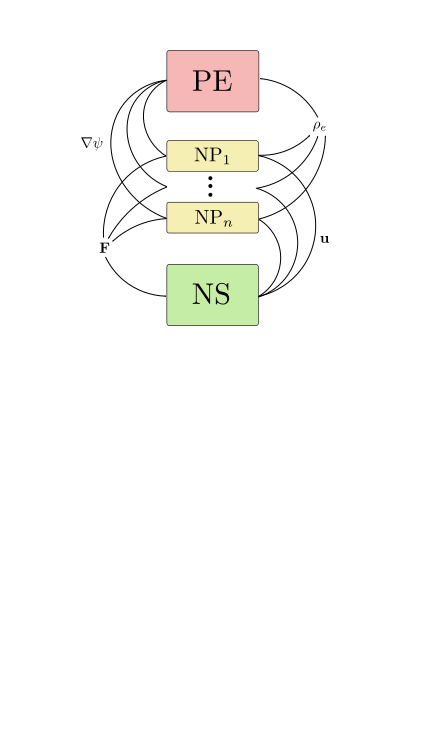
\includegraphics[width=0.5\textwidth]{fig/coupling.pdf}
\end{center}
\caption[Visualisation of the coupling between the equations
  present in the model.]{Visualisation of the coupling between the
  three equations present in the model. Poisson's equation (PE), the
  set of Nernst-Planck equations (NP$_1$ ... NP$_n$) for the different
  ion species and the Navier-Stokes equations (NS). The dependencies
  have also be marked with arrows indicating what quantities for a
  certain equation that are needed from an other.}
\label{fig:coupling}
\end{figure}

%The algorithm to solve the coupled equations is described in section
%\ref{lb:algorithm}.



\section{The potential - Poisson's equation}\label{sec:et:poisson}
To be able to model the flow dynamics of liquids in a channel with
present EDLs, the potential and charge distribution
in the channel must be determined. These quantities are mutually
related through Poisson's equation for electrostatics:

\begin{equation}\label{eq:pb}
\nabla^2\psirm = -\frac{\rho_e}{\epsilon_r \epsilon_0}
\end{equation}
where $\psirm$ is the electrical potential, $\rho_e$ the electrical
charge density, $\epsilon_r$ is the relative permittivity and
$\epsilon_0$ the vacuum permittivity. Under certain assumptions, the
charge density may be explicitly determined as a function of the
potential distribution, one such result is the so called
Poisson-Boltzmann equation, further discussed in section \ref{sec:et:pb}.

\subsection{Boundary conditions}
At the charged boundaries, most physical situations may be covered by
either specifying the potential or the surface charge density. The
former would be a boundary condition of Dirichlet type:

\begin{equation}
\psirm(\x) = \zeta(\x)\;,\;\; \x \in \Gamma
\end{equation}
and the latter a boundary condition of Neumann type:

\begin{equation}\label{eq:et:fix_c}
\nabla\psirm(\x) \cdot \n =
-\frac{\sigma(\x)}{\epsilon_0\epsilon_r}\;,\;\; \x \in \Gamma
\end{equation}
where $\Gamma$ denotes the boundary of the domain and $\n$ is the
normal to the boundary surface.\- \cite{hlushkou}


\section{The transport of charges - Nernst-Planck equation}\label{sec:et:np}
The charge concentration in an electrolyte is indeed affected by its
environment. In the model proposed here, influences from: advection of
the electrolyte, diffusion due to concentration gradients and effects
from the electric field originating from charged objects placed at the
border or in the flow is considered. Charge conservation without any
external sources of the ion density, $\C(\x, t)$, gives:

\begin{equation}\label{eq:charge_conc}
\dfrac{\partial \C}{\partial t} + \nabla \cdot \J = 0
\end{equation}
where $\mathbf{J(\mathbf{x}, \mathrm{t})}$ is the net flux induced
by the effects described above. Explicit expressions for the fluxes
due to advection and diffusion respectively are 

\begin{equation}
\J_{adv} =
\C\ubf
\end{equation}
and 
\begin{equation}
\mathbf{J}_{dif} = -D\nabla \C 
\end{equation}
where $\mathbf{u}$ is the advective velocity and $D$ is a diffusion
coefficient. The ionic flux due to the presence of an electric
potential, $\psirm(\x, t)$, is given by the Nernst equation
\cite{dongquing-ren-book}:

\begin{equation}
\J_{ele} = -\frac{zq_eD}{k_BT}\C\nabla\psirm
\end{equation}
where $z$ is the relative charge of the ion species, $q_e$ is the
fundamental charge, $k_B$ is the Boltzmann constant and $T$ is the
temperature of the fluid.

Summing up the fluxes and putting them into eq. \eqref{eq:charge_conc}
gives

\begin{equation}\label{eq:et:np}
\dfrac{\partial \C}{\partial t} = \nabla \cdot \left [
 D\nabla \C - \C\ubf + \frac{zq_eD}{k_BT}\C\nabla\psirm
\right]
\end{equation}
which is a known result often referred to as the Nernst-Planck
equation. This is the equation for the transport of \emph{one} species
of ions, if several are present one NP equation for each species needs
to be solved. The advective velocity, $\ubf$, and the potential
gradient, $\nabla \psirm$, are obtained from couplings to the
Navier-Stokes and Poisson's equation respectively. More about the
coupling between the equations is discussed in section
\ref{sec:et:coupling}.

\subsection{Boundary conditions}
Depending on the physical situation being modelled, different
conditions may be imposed at the boundaries of the domain. Throughout
this work, at hard boundaries (walls), the charge flux through the
boundary is set to zero, i.e.:

\begin{equation}\label{eq:et:j0}
\J \cdot \mathbf{n} = 0 \;,\;\; \x \in \Gamma
\end{equation}
where $\mathbf{n}$ denotes the normal to the surface and $\Gamma$ is
the boundary of the domain. 


%what we need

%nernst planck


%poisson boltzmann steady state, fix potential 

\subsection{Poisson-Boltzmann equation}\label{sec:et:pb}
Consider a system consisting of an electrolyte in contact with a
(flat) charged wall.  Under certain assumptions, it is possible to
explicitly determine the charge density in eq. \eqref{eq:et:np} as a
function of the electric potential. E.g. if there is no advection
present and if the system has reached a steady state, i.e. $\partial
\C /\partial t = 0$ and $\ubf = \mathbf{0}$ we have:

\begin{equation}\label{pb_constant_flux}
D\nabla \C + \frac{zq_eD}{k_BT}\C\nabla\psirm = \J_0
\end{equation} 
where $\J_0$ is a constant flux. Due to the steady state
assumption, what the equation above actually says is that the net flux
of charge in the system is constant. Since no charges are wanted to
flow through the wall boundary, the flux is set to zero on the wall
and since the flux is constant it will therefore be zero everywhere in
the liquid, i.e. $\J_0 = 0$.

Considering only a one-dimensional situation with a position variable
$y$ varying in a direction out from the wall into the liquid,
eq. \eqref{pb_constant_flux} reads

\begin{equation}\label{eq:pb_eq_for_C}
\frac{1}{\C} \dfrac{d \C}{d y} + \frac{zq_e}{k_BT} \dfrac{d \psirm}{d
  y} = 0.
\end{equation}

The charge density is determined by solving eq. \eqref{eq:pb_eq_for_C}
for $\C$, i.e. integrating the equation. In order to avoid introducing
additional unknown quantities, the equation is integrated to far away
from the wall where the potential from the EDL is assumed to have
decreased to zero and where the concentrations, $\C^{\infty}$, of the
electrolyte is known.

\begin{equation}
\int_y^{\infty} d\ln( \C(y')) = -\frac{z q_e}{k_BT}\int_y^{\infty}d\psirm(y')
\end{equation}
This gives an expression for $C(y)$:

\begin{equation}\label{eq:C}
\C(y) = \C^{\infty} \exp\left(-\frac{z q_e \psirm(y)}{k_BT}\right).
\end{equation}

In a general case, there may be several species of ions in the
electrolyte, the net charge density, $\rho_e$, is then given by simply
summing up the contributions from the different species:

\begin{equation}\label{eq:rho}
\rho_e = q_e\sum_i z_i \C_i.
\end{equation}

Summarising eqs. \eqref{eq:pb}, \eqref{eq:C} and \eqref{eq:rho} gives
the Poisson-Boltzmann equation in one dimension

\begin{equation}\label{eq:pb_real}
\dfrac{d^2\psirm(y)}{dy^2} = -\frac{q_e}{\epsilon_r \epsilon_0}\sum_i z_i
\C_i^{\infty} \exp\left(-\frac{z_i q_e \psirm(y)}{k_BT}\right).
\end{equation}

\subsubsection{The Debye–Hückel approximation}
Historically, the non-linear nature of eq. \eqref{eq:pb_real}
complicated for those wanting to solve it. This was a major difficulty
in the past when the computational power at hands were rather
limited. A linearisation is therefore sometimes done, this linear
version of the PB equation is often referred to as the Debye–Hückel
approximation. The solution of the linearisation gives, something to
compare with and is usually used when defining a characteristic length
scale of the EDL.

For a 1:1 electrolyte solution with an equal amount of positive and
negatively charged ions, eq. \eqref{eq:pb_real} reduces to

\begin{equation}
\frac{d^2\psi(x)}{dx^2} = \frac{2\C^{\infty}q_ez}{\epsilon_r
  \epsilon_0}
\sinh\left(\frac{z q_e \psi(x)}{k_BT}\right).
\end{equation}
and the linearised equation is

\begin{equation}
\frac{d^2\psi(x)}{dx^2} = \frac{2\C^{\infty}q_e^2z^2}{\epsilon_r
  \epsilon_0 k_B T} \psi(x) = \kappa^2 \psi(x)
\end{equation}
where $\kappa^{-1}$ is the Debye length which is where the exponential
solution has decayed to $e^{-1}$ of the boundary value. This quantity
gives therefore a measure for the characteristic thickness of the EDL.

\nomenclature{PB, P-B}{Poisson-Boltzmann model/equation}
%% In this work, flows of ionic solution will be studied and the
%% assumption with thermodynamical equilibrium does not apply. However
%% for low-speed flows the model may still be a decent approximation,
%% which will be investigated.

%% The second assumption, may also stay unfulfilled in some cases
%% investigated here. The fluid in contact with the wall must be of
%% substantial size in relation to the EDL thickness. There will be
%% cases where the choice of $\zeta$ potential in combination with thin
%% channels will make this assumption not fulfilled.

%% Since the PB equation is unable to model the system of
%% interest, a different approach will be presented. However, throughout
%% this work, references and comparisons with the PB model w
%% ill be made. 


%intro

%liten härledning av högerledet 
%diffusion by conc grad. = grad of
%potential <==> termodynamic equilibrium
%chem pot definerad som....
% eq.
% boundary conditions
%antagaganden !!!


%% A simple and commonly used approach for determining potentials (and
%% charge distributions) in systems with present EDLs is by solving
%% eq. \eqref{eq:pb} with a charge distribution of Boltzmann
%% type. Here follows a brief derivation of this term together with some
%% discussion on the assumptions made.

%% The fundamental assumption that the derivation of the charge
%% distribution is based on, is the fact that the system is assumed to be
%% under thermodynamical equilibrium. I.e. forces, acting on the ions,
%% due to chemical diffusion from concentration gradients and from the
%% electrical field are therefore balancing each other. In one dimension:

%% \begin{equation}\label{eq:dif_elec_forces}
%% \frac{d \mu_i}{dx} = -z_i q_e\frac{d\psi}{dx}
%% \end{equation}
%% where $\mu_i$ is the chemical potential for species $i$, $z_i$ is the
%% relative charge of species $i$, $q_e$ the fundamental charge and
%% $\psi$ is the EDL potential. The chemical potential is given by
%% \cite{ren}:

%% \begin{equation}
%% \mu_i = \mu_i^{\infty} + k_BT\ln n_i
%% \end{equation}
%% where $\mu_i^{\infty}$ is a reference value for the chemical potential,
%% here the potential value far from the charged wall is used, $k_BT$ is
%% the thermal energy and $n_i$ is the ion concentration of species
%% $i$. This expression plugged into eq. \eqref{eq:dif_elec_forces} gives

%% \begin{equation}\label{eq:eq_for_ni}
%% \frac{d \ln(n_i)}{dx} = - \frac{z_i q_e}{k_BT}\frac{d \psi}{dx}.
%% \end{equation}


\section{The velocity field - Navier-Stokes equations}\label{sec:et:ns}
The Navier-Stokes equations are among the most fundamental corner
stones of hydrodynamics. They describe the motion of a fluid under
the influence of various internal and external forces.

For later convenience and for reference when it comes to deriving the
Lattice-Boltzmann formulation of the NS equation, a brief sketch of a
derivation will here be presented. A most general form of the
Navier-Stokes equation follows from momentum conservation

\begin{equation}
\dfrac{\partial (\rhorm \ubf)}{\partial t} + \nabla \cdot (\rho \ubf
\otimes \ubf) + \Q = 0 
\end{equation}
where, $\rhorm$ is fluid density, $\ubf$ is velocity, $\otimes$
represents the outer product and $\Q$ is a momentum source term
(force per volume). Expanding the time derivative and the divergence
terms respectively gives
 
\begin{equation}\label{eq:et:nspre}
\ubf \left ( \dfrac{\partial \rhorm}{\partial t} + \nabla \cdot
  (\rhorm \ubf) \right ) + \rhorm \left (\dfrac{\partial \ubf}{\partial t} +
  \ubf \cdot \nabla \ubf 
  \right ) + \Q = 0.
\end{equation}
To assure mass conservation (without sources) we have

\begin{equation}\label{eq:et:mass_conc}
 \dfrac{\partial \rhorm}{\partial t} + \nabla \cdot(
  \rhorm \ubf) = 0
\end{equation}
and eq. \eqref{eq:et:nspre} reduces to

\begin{equation}\label{eq:et:ns_general} 
\rhorm \left (\dfrac{\partial \ubf}{\partial t} +
  \ubf \cdot \nabla \ubf 
  \right ) + \Q = 0
\end{equation}
which together with eq. \eqref{eq:et:mass_conc} is a general
formulation of the Navier stokes equations. 

The force term $\Q$, is determined by the physical properties of the
fluid and from its environment. In this work, only incompressible
($\rho = \mbox{constant}$) Newtonian fluids will be studied. The force
contribution to $\Q$ involved in that case is limited to viscous
forces, pressure gradients in the fluid and to external force
fields. Putting this into eqs. \eqref{eq:et:mass_conc} and
\eqref{eq:et:ns_general} gives

\begin{equation}\label{eq:et:ns_incompressible}
 \nabla \cdot \ubf = 0
\end{equation}
and

\begin{equation}\label{eq:et:ns_mom}
\rhorm \left (\dfrac{\partial \ubf}{\partial t} +
  \ubf \cdot \nabla \ubf 
  \right ) = - \nabla \Prm  + \mu \nabla^2 \ubf + \F
\end{equation}
where $\Prm$ is the pressure, $\mu$ the kinematic viscosity and $\F$
is the contributions from  external forces.

\subsection{Boundary conditions}

At hard boundaries (walls), the boundary conditions to
eqs. \eqref{eq:et:ns_incompressible} and \eqref{eq:et:ns_mom} are set
on the velocity of either a Dirichlet or Neumann type. In most
physical situations the Dirichlet condition is used which corresponds
to that there is a friction between the fluid and the wall, usually
full friction, i.e. when no relative movement between fluid and wall
is present and the velocity at the wall boundary is set to zero, i.e.

\begin{equation}
\ubf = 0 \;,\;\; \x \in \Gamma
\end{equation} 
where $\Gamma$ denotes the boundary. The Neumann type conditions are
used for no-friction walls where the normal component of the
derivative of the velocity is specified, usually to zero.

At wet boundaries, inlets and outlets, of the domain various boundary
conditions may be set. For instance the pressure or the velocity could
be fixed. In the case of a fixed pressure boundary, a flow direction
must also be specified for completeness. \cite{he_zou}


\section{Pressure-driven electrokinetic flow}\label{sec:et:streaming_pot}
As a charged fluid is driven by a pressure gradient, a movement of
charges, i.e. an electrical current will be induced. Due to the charge
flux, a potential gradient will build up along the flow
direction. This potential is usually referred to as the streaming
potential, $\phi(\x)$, and its magnitude is determined from the
induced current through Ohm's law

\begin{equation}
\J = -  \sigma \nabla \phi  
\end{equation}   
where $\sigma$ is the conductivity of the fluid. in a perfectly
conducting fluid there will be no potential differences. Also a
complete neutral solution will carry no net current and also in this
case there will be no potential differences.

Charges under the influence of an electric field will be affected by a
force. Charges moving due to this force will, in a liquid, also pull
liquid (uncharged) molecules with them. In a macroscopic limit, the
force density affecting the charges in the liquid is assumed to affect
the liquid as a whole. The volumetric force affecting the fluid from
the presence of the streaming potential is then given by:

\begin{equation}
\F = - \rho_e \nabla \phi
\end{equation}
where $\rho_e$ is the charge density. This is an example of how the
charge density from the Nernst-Planck equation may couple to the force
term in Navier-Stokes equations. 

This force will always be affecting the fluid in a direction opposite
to the net flux of charge, i.e. the force will slow the fluid down,
this is illustrated in fig. \ref{fig:et:ev}. This effect that a moving
net charged fluid is slowed down is called the \emph{electroviscous
  effect}. The name originates from that a similar effect might be
achieved by increasing the viscosity of the fluid.

\begin{figure}
\begin{center}
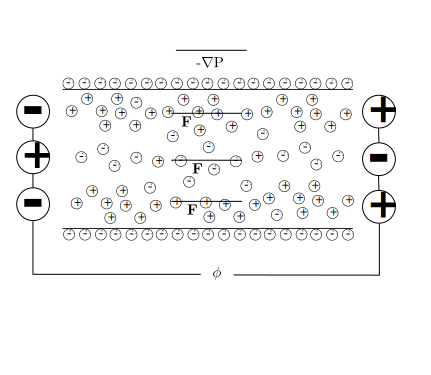
\includegraphics[width=0.7\textwidth]{fig/channel_electroviscous.pdf}
\end{center}
\caption[Example of an electroviscous system.]{Example of an
  electroviscous system. The fluid is driven by a pressure gradient,
  $\nabla \Prm$. The directions of the forces on the fluid are always
  opposite to the flow direction. The force originates from the
  potential difference, $\phi$, that builds up along the channel. The
  force is always opposite to the flow direction, thus slowing the
  flow down.}
\label{fig:et:ev}
\end{figure}


\section{Electroosmotic flow}\label{sec:et:electroosmosis}
Instead of driving the fluid flow through a pressure drop, a net
charged fluid may be driven by an external electric field. This may
be seen as the opposite case to that in section
\ref{sec:et:streaming_pot} where a current is induced by a pressure
drop.

The volumetric force on the fluid from the external field, $\E_{ext}$,
is given by

\begin{equation}
\F = \rhorm_e \E_{ext}
\end{equation}

where $\rho_e$ is the charge density. If the electric field is
constant (or at least has the same direction) everywhere, the sign of
the force is not in the same direction for a net charged positive area
of the fluid as for a net charged negative. Thus the fluid may be
either slowed down or sped up. This is a qualitative difference to
pressure driven situation and is illustrated in fig. \ref{fig:et:eo}.

\begin{figure}
\begin{center}
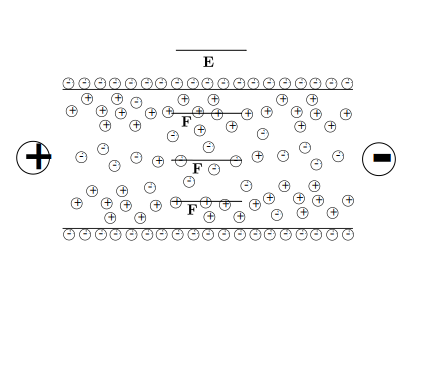
\includegraphics[width=0.7\textwidth]{fig/channel_electroosmosis.pdf}
\end{center}
\caption[Example of an electroosmotic system.]{Example of an
  electroosmotic system. The fluid is driven by an external electric
  field, $\E$. The directions of the forces on the fluid from the
  electric field are indicated with arrows. Note however that the
  fluid does not necessarily has to flow in the direction of the
  force, this due to viscous effects in the fluid. }
\label{fig:et:eo}
\end{figure}

The electroviscous effect is in the case of pure electroosmotic flow
usually neglected as the field due to the streaming potential is, in
most physical cases, small in comparison to the applied external
field. \cite{wang-poi}


%lite intro

%börja inte med allmän teoretisk formulering

%sedan lite resultat, double layers

%pressure driven flows...


\chapter{The lattice-Boltzmann method}\label{sec:lbm}
Rather than modelling on a macroscopic or microscopic scale, the
lattice-Boltzmann method (LBM) operates at a scale in between those,
often referred to as a mesoscopic scale. Nowadays, the method is most
frequently used in modelling of fluid dynamics, i.e. computing
solutions of the macroscopic Navier-Stokes equations. However, the
lattice-Boltzmann method is not limited to this case and may be used
to model other macroscopic systems as well. In this chapter a LBM
approach will, in addition to the Navier-Stokes equations, also be
formulated for the Nernst-Planck and Poission's equation.

\nomenclature{LBM}{Lattice-Boltzmann Method}

\section{Historical overview}
With the introduction of electronic calculating machines came also
completely new possibilities of tackling difficult problems. New
fields of computational science was born and methods for solving both
new and traditional problems were developed.

The idea of using a discrete and simplified version of the
Boltzmann-equation dates back to the mid 60's \cite{scholarpedia-lbm}
with an experimental attempt to model simple gas dynamics. However, at
the time, this kind of statistical computational approaches was not
considered a serious alternative for the modelling of more
sophisticated and complex systems such as fluid behaviour. It was
first in the mid 80's when Frisch, Hasslacher and Pomeau showed that a
lattice automaton that conserved mass and momentum in the collisions
and with a lattice of certain symmetry, reproduced the Navier-Stokes
equations in a macroscopic limit. It was by their work and the always
increasing computational power that made the idea of fluid modelling
on a mesoscopic scale a serious research topic. \cite{wolf-gladrow}

The lattice gas automata (LGA) approach was not perfect and suffered
from some notable flaws, e.g. that the boolean nature of the method
introduced statistical noise and that lack of symmetry in the lattices
used made the advection non-isotropic. The statistical noise was
usually dealt with by averaging which resulted in a coarsed domain and
the advection issue was handled by introducing lattices of higher
symmetry. An other consequence of the boolean variables is that only one
particle per state was allowed which resulted in an equilibrium state
from Fermi-Dirac statistics rather than the desired Maxwell-Boltzmann
statistics. 

As the flaws of the LGA approach was resolved one by
another, the method evolved into what we today know as the
lattice-Boltzmann method, with the crucial refinement of using
continuous distributions over boolean variables. \cite{wolf-gladrow}

Today, the lattice-Boltzmann method is in many situations indeed a
competitor to more traditional CFD methods. For example with
advantages when it comes to parallelisation or implementing boundary
conditions in complex geometries. One major downside with the LBM is
the lack of theoretical work done and lack of literature compared to
the case with more traditional methods such as finite element/volume
methods. \cite{junk-asym}

\nomenclature{LGA}{Lattice Gas Automata/Automaton}
\nomenclature{CFD}{Computational Fluid Dynamics}


\section{Statistical background}\label{sec:lbm:stat}
Consider one litre of air. At STP, the volume will contain in the
order of $10^{22}$ molecules. In order to model this system
microscopically, 6 variables per molecule will be needed to describe
the microstate of the system. Just to store the state of the system in
a computer would require more space than the estimated size of the
whole world wide web times one million \cite{wolfram-alpha-web}. Thus,
for these kind of systems, the microscopic approach is somewhat
impractical.

\nomenclature{STP}{Standard Temperature and Pressure}

Statistical approaches have been developed for these types of
problems. A fundamental quantity used for describing the system is a
continuous probability density distribution, $f$. This distribution
may be regarded as an average over the microstates. Consider a volume
of $d^3\x d^3\mathbf{p}$ in phase space, the number of molecules, $dN$
in this volume is then given through the density distribution, $f$ as

\begin{equation}
dN(\x, \p, t) = f(\x, \p, t)\drm^3\x \drm^3\p.
\end{equation}
Thus $f(\x, \p, t)$ is a measure of the number of particles at
location $\x$ with momentum $\p$ and at time $t$. Macroscopic variables are
obtained by summing, e.g. the particle density, $n$, is obtained from

\begin{equation}
n(\x, t) = \int f(\x, \p, t) \drm^3\p
\end{equation}
and the macroscopic momentum density of the system is determined by

\begin{equation}
\rho(\x, t) \ubf(\x, t) = \int \p f(\x, \p, t) \drm^3\p
\end{equation}
where $\rho = m n$ is the mass density. Multiplying $f$ by a power $k$ of
$\p$ or $\mathbf{v} = \p/m$ and integrating is often referred to as
taking the $k$:th moment of $f$ and is a term that will be used
throughout this chapter.

In the late 19th century, Boltzmann developed a model for the time
evolution of $f$. To do this he had to make several
assumptions. First, only collisions between two particles are
considered, this makes the equation mostly applicable to dilute
gases. Second, the two particles colliding are assumed to be
uncorrelated before the collision. Third, external forces are assumed
not to affect the collisions \cite{wolf-gladrow}. The equation is
named after its father to the Boltzmann (transport) equation and
reads:

\begin{equation}\label{eq:lbm:boltzmann-eq}
\partial_t f + \frac{\p}{m} \cdot \nabla_{\x}f + \frac{\F}{m} \cdot
\nabla_{\mathbf{v}}f = Q(f, f)
\end{equation}
where $f$ is the distribution function for a single species collection
of particles of mass $m$, $\F$ is external forces, $\p$ is momentum,
$\nabla_{\x}$ and $\nabla_{\mathbf{v}}$ are the gradients in location
and velocity space respectively. The right-hand side contains the so
called collision term which in the general case is expressed as an
integral. This integral states how the distribution function changes
after a two particle collision. However, the structure of this
integral is in most physical situations too complicated to be used
directly. Therefore, a number of simplifications have been proposed
during the years.

When designing these approximations, at least two main properties of
the collision integral must be kept. \cite{wolf-gladrow}

\begin{enumerate}
  \item The same quantities that are conserved under collisions in the
    collsion integral must also be conserved in the approximation.
  \item Boltzmann's H-theorem must be fulfilled for the
    approximated collision operator.
\end{enumerate}

Without being to specific, the H-theorem states that the entropy
computed from $f$ is always increasing with time and that the maximum
entropy is obtained for a so called Maxwellian distribution in
momentum/velocity space. Boltzmann used an other quantity denoted by H
closely related to entropy, thus the name of the theorem. The
Maxwellian distribution in two dimensions that $f$ tends towards is
given by

\begin{equation}\label{eq:lbm:maxwell}
f^{(M)}(\x, \mathbf{v}, t) = n \left ( \frac{m}{2 \pi k_B T} \right )
\exp{\left( -\frac{m}{2 k_B T} (\mathbf{v} - \ubf)^2\right)}
\end{equation} 
where $\ubf(\x, t)$ is the mean velocity of the particles in the system and
$n(\x, t)$ is the number of particles at location $\x$. In section
\ref{sec:lbm:col}, one of the most widely used approximations of the
collision integral will be presented.


\section{Basic idea of the LBM}
As previously noted, the lattice-Boltzmann method is a mesoscopic
method. This means that the modelling is neither done on a microscopic
(molecular) level nor by direct solving of the macroscopic equations
involved. The aim, in most situations with the lattice-Boltzmann
method is indeed to solve some macroscopic equation but not
direct. Instead a statistical model is used with various mesoscopic
variables that, in some limit, reproduces the macroscopic
variables. It is also possible to ensure that these variables (to some
extent) fulfil a certain macroscopic equation by using a certain
scheme.

Basically the lattice-Boltzmann method solves a discretised version of
eq. \eqref{eq:lbm:boltzmann-eq} for the distribution functions from
which the macroscopic quantities may be determined. Both the spatial
positions and the velocity space is discretised allowing the
distributions to ``sit'' only at certain positions and to stream to
neighbouring locations only in certain directions. A naive way to
visualise the evolution of $f$ is to consider the distribution
functions at the lattice nodes as pseudo particles that move along the
lattice and collide.

Usually in two dimensions the velocity space is discretised into 9
distinct velocities, more about the choice of lattice is discussed in
section \ref{sec:lbm:lattice}. In this case 9 distribution functions
are needed per node which might correspond to one or two macroscopic
variables but is indeed fewer than the number of variables needed for
a microscopic approach.

The discretised Boltzmann equation is referred to as the
lattice-Boltzmann equation (LBE) and is one of the fundamental corner
stones in the lattice-Boltzmann method, it reads:

\begin{equation}\label{eq:lbm:lbe}
f_i(\x + \cbf_i\delta_t, t + \delta_t) - f_i(\x, t) = \Omega_{ij}(\x, t)
\end{equation}
where $f_i$ denotes the distribution function for direction $\cbf_i$,
$\delta_t$ is the time step and $\Omega_ij$ is the (for now
non-specified) collision operator. An implicit sum over the second
velocity index $j$ is assumed. Various forms of collision operators
exist and will be further discussed in section \ref{sec:lbm:col}.

\subsection{Computational algorithm}
In order to solve eq. \eqref{eq:lbm:lbe} the distribution functions
must be set to some initial value. The choice of initial value is in
most cases crucial with respect to stability and accuracy of the
method. More about the initialisation will be discussed in later
sections of this chapter. 

When a proper initialisation has been performed, the time evolution of
the distribution functions is determined iteratively by the explicit
scheme in the LBE, eq. \eqref{eq:lbm:lbe}. The update in each time
step is usually divided into two computational tasks. First, the new
value that later will be propagated to a neighbouring node is computed,
i.e.

\begin{equation}
f_i^{*}(\x, t + \delta_t) = f_i(\x, t) + \Omega_{ij}(\x, t)
\end{equation}
This step will be referred to as the collision step since it is here
the ``collision'' is computed. The second step consists of propagating
the distribution functions to the neighbouring node in its
corresponding direction, i.e.
\begin{equation}
f_i(\x + \cbf_i\delta_t, t + \delta_t) = f_i^*(\x, t + \delta_t)
\end{equation}
This step will be referred to as the streaming step.

In the case of a finite domain, certain rules (boundary conditions)
must be specified at the boundaries. Typically the distribution
functions that are going to be streamed out of the domain is used to
define the unknown ones that will ``enter'' the domain. More about
boundary conditions in section \ref{sec:lbm:bound}. Thus, at each time
step, the boundary conditions must also be handled. 

This is broadly the whole computational algorithm behind the LBM, in
fig. \ref{fig:lbm:algo}, a flow scheme of the algorithm is shown.

\begin{figure}
\begin{center}

\includegraphics[width=0.5\textwidth]{fig/algorithm.pdf}
\end{center}
\caption[Flowchart of the most fundamental parts in an implementation
  of the LBM.]{Flowchart of the most fundamental parts in an implementation
  of the LBM. The convergence is usually tested for a macroscopic
  variable.}
\label{fig:lbm:algo}
\end{figure}

\nomenclature{LBE}{Lattice-Boltzmann Equation}


\section{The BGK collision operator}\label{sec:lbm:col}
The collision term in the LBE is the main ingredient in what
determines the physics of the system that is being modelled. Here the
desired interaction of the pseudo particles is stated. In section
\ref{sec:lbm:stat}, two necessary properties to approximations of the
full collision integral was stated.

One of the simplest collision operators that fulfil conditions (1)
and (2) in section \ref{sec:lbm:stat} is the BGK operator (BGK from
its creators: Bhatnagar, Gross and Krook). It was proposed in 1954 and
is today one of the most commonly used collision operators both in the
case of the lattice-Boltzmann and the continuous Boltzmann
equation. It is based on the principle of relaxing $f$ towards a
Maxwellian distribution. The relaxation is also performed in such a
way that the collision invariants are preserved.  In the discrete case,
eq. \eqref{eq:lbm:lbe}, the operator is given by:

\begin{equation}\label{eq:lbm:bgk}
\Omega_{ij} = \Omega_i = -\omega \left[ f_i(\x, t) - f_i^{(eq)}(\x, t)
  \right]
\end{equation}
where $\omega$ is a parameter determining the relaxation rate and
$\feq$ should be an equilibrium distribution that makes sure that the
necessary conditions are fulfilled. In the discrete case, a truncated
expansion of eq. \eqref{eq:lbm:maxwell} is typically used
\cite{wolf-gladrow}. This gives for instance


\begin{equation}
\feq = w_i\rho \left [ 1 + \frac{\ci \cdot \ubf}{c_s^2} +
  \frac{(\ci \cdot \ubf)^2}{2c_s^4} - \frac{\ubf^2}{2c_s^2} \right]
\end{equation}
where $w_i$ is a lattice specific weight, $\rho$ is the zeroth moment
of $\fii$ and $\ci$ is a unit velocity in the discretised velocity
space.

The BGK operator is due to its simplicity both when it comes to
theoretical treatment and implementation a popular choice. However in
some physical situations, e.g. multi-phase or high Reynolds-number
flows, more sophisticated alternatives are required
\cite{wolf-gladrow}. Throughout this work, the BGK operator will be
used.

\nomenclature{BGK}{Relaxation type collision operator (Bhatnagar,
  Gross and Krook)}


\section{The lattice}\label{sec:lbm:lattice}
The discrete spatial coordinates together with the discrete velocity
coordinates forms a lattice. Spatial coordinates are neighbourwise
connect through the discrete velocities. The discretisation in the LBM
must be performed in such a way that the lattice may be produced from
translating a single unit cell. This gives that the spatial resolution
is constant for the whole domain. In other approaches, e.g. finite
element methods the mesh may locally be refined at interesting regions
of the domain which is a strength to these methods over the LBM.  

There exist a convention for naming different lattices. A lattice of
dimension $d$ and with $q$ distinct velocities is denoted by
D$d$Q$q$. For example a lattice with 9 velocities in dimension 2 is
denoted D2Q9. An example of two different lattices is presented in
fig. \ref{fig:lbm:lattices}. The D2Q9 lattice is also the one that
will be used in this work, the velocities $\ci$ are given by

\begin{equation}\label{eq:lbm:d2q9_c}
\{\ci\} = \left\{
\begin{bmatrix}0\\0\end{bmatrix}, 
\begin{bmatrix}1\\0\end{bmatrix}, 
\begin{bmatrix}0\\1\end{bmatrix}, 
\begin{bmatrix}-1\\0\end{bmatrix}, 
\begin{bmatrix}0\\-1\end{bmatrix}, 
\begin{bmatrix}1\\1\end{bmatrix}, 
\begin{bmatrix}-1\\1\end{bmatrix}, 
\begin{bmatrix}-1\\-1\end{bmatrix}, 
\begin{bmatrix}1\\-1\end{bmatrix}
\right\} 
\end{equation}

\begin{figure}
  \centering
  \subfloat[D2Q7
    ]{\label{fig:lbm:q7}\includegraphics[width=0.4\textwidth]{fig/lattice_d2q7-crop.pdf}}      
  \hspace{15pt} \subfloat[D2Q9
  ]{\label{fig:lbm:q9}
\includegraphics[width=0.35\textwidth]{fig/lattice_d2q9.pdf}
  }
  \caption[Two different unit cells for lattices used in the LBM in two
    dimensions.]{Two different unit cells for lattices used in the LBM in two
    dimensions. In (a) the D2Q7 seven speed lattice is shown and in
    (b) the nine speed D2Q9 lattice. The numbering at the edges is the
    usual naming convention for the different velocities.}
  \label{fig:lbm:lattices}
\end{figure}
 
To be able to retrieve the desired equations in the macroscopic limit
of the LBE, the lattice used must possess a certain degree of
isotropy. Thus the choice of lattice is not arbitrary. For instance,
for obtaining the Navier-Stokes equations, the lattice velocities must
at least posses the following properties:

\begin{subequations}\label{eq:lbm:i0}\label{eq:lbm:i1}\label{eq:lbm:i2}\label{eq:lbm:i3}\label{eq:lbm:i4}
\begin{align}
\sum_i w_i &= 1\\
\sum_i w_ic_{i\alpha} &= 0 \\
\sum_i w_ic_{i\alpha}c_{i\beta} &= c_s^2\delta_{\alpha \beta}\\
\sum_i w_ic_{i\alpha}c_{i\beta}c_{i\gamma} &= 0\\
\sum_i w_ic_{i\alpha}c_{i\beta}c_{i\gamma}c_{i\delta} &= c_s^4(\deltasec)
\end{align}
\end{subequations}

%\begin{equation}\label{eq:lbm:i5}
%\sum_i w_ic_{i\alpha}c_{i\beta}c_{i\gamma}c_{i\delta}c_{i\kappa} = 0
%\end{equation}

where the sums are over the discrete velocities $\ci$, $w_i$ are
lattice specific weights $c_s$ is the speed of sound for the lattice
and $\delta_{ij}$ is a Kroenecker delta. 

The weights are introduced to compensate for the fact that different
velocity vectors are of different length. See for example the
D2Q9 lattice in fig. \ref{fig:lbm:q9} where three lengths are
present. In this case, three different weights will be needed. From
the relations in eqs. \eqref{eq:lbm:i1} follow that
these weights are: 
\begin{equation}\label{eq:lbm:weights}
w_i = 
\left\{
  \begin{array}{l l}
    4/9 & \quad \text{if $i = 0$}\\ 
    1/9 & \quad \text{if $i = 1, 2, 3, 4$}\\    
    1/36 & \quad \text{if $i = 5, 6, 7, 8$}\\
  \end{array} \right.
\end{equation}
The quantity $c_s$ which often is referred to as the speed of sound
may be thought of as an effective propagation velocity of the lattice
and is determined, for the D2Q9 lattice, to

\begin{equation}
c_s = c/\sqrt{3}
\end{equation} 
where $c = |\mathbf{c}_{1,2,3,4}| = \delta_x/\delta_t$.

\nomenclature{D2Q9}{2D lattice with 9 discrete velocities}


\section{Asymptotic analysis}\label{sec:lbm:asym}
Methods from asymptotic analysis will, in this section, be used to
investigate the macroscopic limit of the general LBE. More detailed and
specific analyses for the three different equations considered will be
presented in sections \ref{sec:lbm:asym_np}, \ref{sec:lbm:asym_ns} and
\ref{sec:lbm:asym_pe} respectively. 

Asymptotic analysis is basically about describing mathematical objects
in some limit, e.g. how a function behaves for large or small values
of some variable or parameter. Consider for example the series $S_{\ep}$:

\begin{equation}
S_{\ep} = a^{(0)} + a^{(1)}\epsilon + a^{(2)}\epsilon^2 +
a^{(3)}\epsilon^3 + \mathcal{O}(\epsilon^4)
\end{equation}
It is clear that for sufficiently small values of $\epsilon$, the
terms of higher order is of negligible magnitude to those of lower
order and the series may be truncated at some point and still be a
good approximation of $S_{\ep}$. For example if $\ep$ is small, then
$S_{\ep} \approx a^{(0)}$ and we say that if $a^{(1)} \neq 0$ that
this approximation is of first order accuracy.

There are different approaches to go from the discrete LBE to a
continuous macroscopic equation. The most frequently applied one to
obtain the Navier-Stokes equations is the Chapman-Enskog method
\cite{junk-boundary}, which will reproduce the compressible
equations. Another method, often employed by M. Junk and his
associates, e.g. in \cite{junk-asym}, is a method based on regular
asymptotic expansions, this is also the method that will be utilised
in this work and will in the case of Navier-Stokes reproduce the
incompressible equations. A brief discussion of the differences
between the Chapman-Enskog and the regular expansion approaches will
be carried out at the end of this chapter.

The basic idea behind the analysis is to expand the distribution
function $\fii$ in some small parameter, $\epsilon$. Also this
parameter will be related to the spatial and time scales. The
macroscopic limit is obtained by taking the Taylor expansion of the
discrete LBE and comparing terms of equal order in
$\epsilon$. Together with the fact that certain quantities are
invariant under collisions, macroscopic differential equations are
obtained. Now follows the part of the analysis which is common for the
three equations, the more equation specific analysis is carried out in
sections \ref{sec:lbm:asym_np}, \ref{sec:lbm:asym_ns} and
\ref{sec:lbm:asym_pe} respectively.

\subsection{Motivation of the choice of expansion parameter}
A most desired property of the expansion parameter is that it should
be a small and dimensionless number. If the lattice is dense enough with
respect to the characteristic length scale of the system, a suitable
choice is the Knudsen number, $\ep$, which is defined as the ratio of
the mean free path, $\delta_x$, and the characteristic length of the
system under consideration, $\ell_0$, i.e. $\epsilon = \delta_x
/\ell_o$. To be able to perform the asymptotic analysis we must also
relate the time scale to this parameter. From the fact that the
lattice speed $c = \delta_x/\delta_t$ and by introducing a
characteristic speed, $u_o = \ell_0/t_0$, we have

\begin{equation}\label{eq:lbm:rel}
\epsilon = \frac{\delta_x}{\ell_0} = \frac{c}{u_0}\frac{\delta_t}{t_0}
\end{equation}
It is now clear that what determines the relation between the
timescale and the parameter $\epsilon$ is the ratio of the
characteristic speed and the lattice speed which is usually referred
to as the Mach number, Ma. In our particular case we will operate in
the incompressible limit, i.e. Ma $\ll$ 1 and a suitable choice is a
small number, thus Ma = $\epsilon$ is chosen \cite{junk-boundary}. The
discretisation of the space and time step is then related through

\begin{equation}
\delta_x'^2 = \delta_t' = \epsilon^2
\end{equation}
where the primes denote dimensionless variables. This particular
scaling is usually referred to as diffusive scaling.

\subsection{Expanding the LBE}
The LBE, eq. \eqref{eq:lbm:lbe}, with dimensionless variables and the
BGK collision operator reads:

\begin{equation}\label{eq:lbm:nodim_lbe}
f_i(\x' + \epsilon \cbf_i', t' + \epsilon^2) - f_i(\x', t') = -\omega \left[
  f_i(\x', t') - f_i^{(eq)}(\x', t') \right].
\end{equation} 
The primes denoting dimensionless variables will, for readability
reasons, from hereon be dropped. If nothing else is stated we always
consider dimensionless variables.

To obtain a differential equation, the difference equation in
eq. \eqref{eq:lbm:nodim_lbe} is Taylor expanded, which gives

\begin{equation}\label{eq:lbm:taylor_lbe}
\ep(\pd\fii) + \ep^2 (\partial_t\fii + (\pd \fii)^2/2 ) + \ep^3
(\partial_t (\pd\fii) + (\pd\fii)^3/6) + \bigO{\ep^4} = 
-\omega \left[
  f_i - f_i^{(eq)} \right]
\end{equation}
Expanding also $\fii$ and $\feq$ in the parameter $\epsilon$:

\begin{equation}\label{eq:lbm:fi_exp}
\fii = \fie{0} + \ep\fie{1} + \ep^2\fie{2} + \ep^3\fie{3} + \bigO{\ep^4}
\end{equation}

\begin{equation}\label{eq:lbm:fi_eq_exp}
\feq = \feqe{0} + \ep\feqe{1} + \ep^2\feqe{2} + \ep^3\feqe{3} +
\bigO{\ep^4}
\end{equation}
and inserting these expressions into eq. \eqref{eq:lbm:taylor_lbe}
gives an equation with terms of varying orders of $\ep$. Separating
this equation in equations of common orders allows for an analysis of
what happens at different scales of $\epsilon$. For the four leading
orders in $\ep$ we have:

\begin{equation}\label{eq:lbm:ep0}
\ep^0:\;\; 0 = -\omega \left[
  \fie{0} - \feqe{0} \right],
\end{equation}

\begin{equation}\label{eq:lbm:ep1}
\ep^1:\;\; \pd\fie{0} = -\omega \left[
  \fie{1} - \feqe{1} \right],
\end{equation}

\begin{equation}\label{eq:lbm:ep2}
\ep^2:\;\; \pd\fie{1} + \partial_t\fie{0} + (\pd \fie{0})^2/2 =
-\omega \left[ \fie{2} - \feqe{2} \right]
\end{equation}
and
\begin{equation}\label{eq:lbm:ep3}
\ep^3:\;\; \pd\fie{2} + \partial_t\fie{1} + (\pd \fie{1})^2/2 +
\partial_t (\pd\fie{0}) + (\pd\fie{0})^3/6 = -\omega \left[ \fie{3} -
  \feqe{3} \right].
\end{equation}

The idea is now that for an equation of a particular order in $\ep$,
use collision invariants and eliminate unknown $\fie{n}$ by using
equations of lower order in $\ep$. This will in the end, result in
differential equations for macroscopic variables, given by moments of
the $\fii$:s.

\nomenclature{CE, C-E}{Chapman-Enskog}


\section{LBM for the Nernst-Planck equation}\label{sec:lbm:np}
The method presented here is based on representing the Nernst-Planck
equation, eq. \eqref{eq:et:np}, as an equation of advection-diffusion
type. Considering the quantity:  

\begin{equation}\label{eq:lbm:eff_adv}
\bar{\ubf} = \ubf -
  \frac{zq_eD}{k_BT}\nabla\psirm
\end{equation}
as an effective advective velocity, we have:

\begin{equation}\label{eq:lbm:adv-dif}
\dfrac{\partial \rho}{\partial t} + \nabla \cdot ( \bar{\ubf} \rho -
  D\nabla \rho ) = 0
\end{equation}
which is a mass conservation equation with fluxes from diffusion and
from advection respectively. The letter $\C$ for denoting the charge
concentration has in this section been replaced by the letter $\rho$
to avoid the risk of confusing it with the lattice velocities
which traditionally are denoted by ${\ci}$.

A collision operator of BGK type, eq. \eqref{eq:lbm:bgk} will be used
together with a D2Q9 lattice. The lattice-Boltzmann equation then
reads:

\begin{equation}
f_i(\x + \cbf_i\delta_t, t + \delta_t) - f_i(\x, t) = -\omega \left[ f_i(\x, t) - f_i^{(eq)}(\x, t) \right]
\end{equation}
with $\{\cbf_i\}_{i=0}^{Q-1}$ for the D2Q9 lattice as in
eq. \eqref{eq:lbm:d2q9_c}. The equilibrium function, $\feq$, is chosen
as \cite{alexey-tobias}:

\begin{equation}\label{eq:lbm:np_feq}
\feq = w_i \rho \left ( 1 + \frac{\ci \cdot \ubar}{c_s^2} \right)
\end{equation}
with the weights, $w_i$, as in eq. \eqref{eq:lbm:weights}. The charge
density and charge flux density is obtained by taking the zeroth and
first moments of the distribution function respectively, i.e:

\begin{equation}\label{eq:lbm:rho_mom}
\rhorm = \sum_i \fii
\end{equation}
and
\begin{equation}\label{eq:lbm:j_mom}
\jj = \sum_i \fii \ci
\end{equation}
The diffusion constant, $D$, is related to the relaxation parameter
$\omega$ through 

\begin{equation}\label{eq:lbm:np_D}
D = c_s^2 \left( \frac{1}{\omega} - \frac{1}{2} \right).
\end{equation}

\subsection{Asymptotic analysis}\label{sec:lbm:asym_np}
To motivate the appearance of the above suggested method for solving
eq. \eqref{eq:lbm:adv-dif} and for showing under what premises the
method is valid, the macroscopic limit of the discrete scheme will now
be analysed in an asymptotic manner. Note that for the advection
diffusion equation mass is but flux is not conserved.

From the expansion of $\fii$ in eq. \eqref{eq:lbm:fi_exp} and from
eqs. \eqref{eq:lbm:rho_mom} and \eqref{eq:lbm:j_mom} follow the
expansions of the mass density and flux respectively as

\begin{equation}\label{eq:lbm:rho_exp}
\rho = \rhoe{0} + \ep\rhoe{1} + \ep^2\rhoe{2} + \ep^3\rhoe{3} + \bigO{\ep^4}
\end{equation} 
and

\begin{equation}
\jj = \je{0} + \ep\je{1} + \ep^2\je{2} + \ep^3\je{3} + \bigO{\ep^4}
\end{equation} 
The advective velocity is also expanded as: 

\begin{equation}
\ubar = \ubare{0} + \ep\ubare{1} + \ep^2\ubare{2} + \ep^3\ubare{3} + \bigO{\ep^4}
\end{equation}
By plugging these expansion into the equilibrium distribution
eq. \eqref{eq:lbm:np_feq}, the expansion in
eq. \eqref{eq:lbm:fi_eq_exp} is obtained. The terms of order zero is
used in the zeroth order equation of the LBE, eq. \eqref{eq:lbm:ep0},
which gives

\begin{equation}
\fie{0} = w_i\rhoe{0} \left( 1 + \frac{\ci \cdot \ubare{0}}{c_s^2} \right).
\end{equation}
However, since we are only considering advection in the low Mach
limit, i.e. $|\ubar| \sim \ep$, we will in this analysis assume that
$\ubare{0} = 0$. $\ubar$ will then be of order $\ep$ to leading
order. It is possible to show \cite{junk-asym} that this assumption
holds if $\ubar$ is initialised properly, i.e. small and if no major
momentum sources are present. Thus the expression for $\fie{0}$
reduces to

\begin{equation}\label{eq:lbm:np_fi0}
\fie{0} = w_i\rhoe{0}.
\end{equation}

We now continue to the equation of order one in $\ep$,
eq. \eqref{eq:lbm:ep1}. Taking the zeroth moment gives the equation $0
= 0$ which indeed is true but not very useful. Note that the right
hand side vanishes due to mass conservation. $\fie{1}$ will be needed
in the next step and is, by using eq. \eqref{eq:lbm:np_fi0}:

\begin{equation}
\fie{1} = -\frac{1}{\omega} (\pd)(w_i\rhoe{0}) + w_i\left( \rhoe{1} +
\rhoe{0} \frac{\ci \cdot \ubare{1} }{c_s^2} \right).
\end{equation}
Taking the first moment of $\fie{1}$ gives the leading order in the
flux ($\je{0} = 0$ since $\ubare{0} = 0$):

\begin{equation}
\je{1} = \rhoe{0}\ubare{1} - c_s^2/\omega\nabla\rhoe{0}
\end{equation} 

Continuing to the equation of order two in $\ep$,
eq. \eqref{eq:lbm:ep2} and taking the zeroth moment of the equation
gives

\begin{equation}
\nabla \cdot \je{1} + \partial_t \rhoe{0} + c_s^2/2\nabla^2 \rhoe{0} = 0
\end{equation}
and by inserting the expression for $\je{1}$ we end up with

\begin{equation}
\partial_t \rhoe{0} + \nabla \cdot \left [ \rhoe{0}\ubare{1} - c_s^2
  \left( \frac{1}{\omega} - \frac{1}{2} \right)\nabla\rhoe{0} \right ]
= 0
\end{equation}
which is an advection diffusion equation with a diffusion constant as
in eq. \eqref{eq:lbm:np_D}. Since $\rhoe{0}$ fulfils the equation of
interest, the solution $\rho$ that we get from the lattice-Boltzmann
method is at least of first order accuracy. To determine the exact
order of accuracy, higher order terms, $\rhoe{k > 0}$, must be
determined. If also all those terms would be zero the method would be
exact, unfortunately that is not the case. The analysis of higher order
terms will not be performed here, but it is possible to show that
$\rhoe{1}$ is zero only under certain premises, i.e. for a proper
initialisation \cite{alexey-tobias}. $\rhoe{2}$ is however in general
non-zero and the obtained solution is thus second order accurate.  


\section{LBM for the incompressible Navier-Stokes}\label{sec:lbm:ns}
The most frequent use of the LBM is to solve the Navier-Stokes
equations. In this work only the incompressible case,
eqs. \eqref{eq:et:ns_incompressible} and \eqref{eq:et:ns_mom} will be
considered. The LBM may however be used to reproduce weak
compressibility \cite{wolf-gladrow}. The incorporation of forces will
be treated in section \ref{sec:lbm:forces}. We recall the
incompressible Navier-Stokes equations without external forces present
from chapter \ref{sec:et} as:

\begin{equation}\label{eq:lbm:ns_inc}
 \nabla \cdot \ubf = 0
\end{equation}
and

\begin{equation}\label{eq:lbm:ns_mom}
\rhorm \left (\dfrac{\partial \ubf}{\partial t} +
  \ubf \cdot \nabla \ubf 
  \right ) = - \nabla \Prm  + \rhorm \nu \nabla^2 \ubf
\end{equation}
where $\nu$ is the kinematic viscosity related through the
dynamic viscosity, $\mu$, by

\begin{equation}
\mu = \rhorm \nu.
\end{equation}

A LBM will now be formulated for eqs. \eqref{eq:lbm:ns_inc} and
\eqref{eq:lbm:ns_mom}. The LBE with a BGK collision operator is given
by

\begin{equation}
f_i(\x + \cbf_i\delta_t, t + \delta_t) - f_i(\x, t) = -\omega \left[ f_i(\x, t) - f_i^{(eq)}(\x, t) \right]
\end{equation}
where

\begin{equation}\label{eq:lbm:ns_eq}
\feq = w_i\rho \left [ 1 + \frac{\ci \cdot \ubf}{c_s^2} +
  \frac{(\ci \cdot \ubf)^2}{2c_s^4} - \frac{\ubf^2}{2c_s^2} \right]
\end{equation}
where $w_i$ are the weights in eq. \eqref{eq:lbm:weights}.

The density, $\rhorm$, and the mass flux, $\rhorm \ubf$, is determined
from $\fii$ by taking the zeroth and first moments respectively:

\begin{equation}\label{eq:lbm:rho_mom}
\rhorm = \sum_i \fii
\end{equation}
and
\begin{equation}\label{eq:lbm:j_mom}
\rhorm \ubf = \sum_i \fii \ci .
\end{equation}
The kinematic viscosity is related to the relaxation parameter,
$\omega$

\begin{equation}\label{eq:lbm:nu}
\nu = c_s^2\left( \frac{1}{\omega} - \frac{1}{2} \right).
\end{equation}

\subsection{Asymptotic analysis}\label{sec:lbm:asym_ns}
Partially based on \cite{junk-asym}, an asymptotic analysis of the
above suggested method will be performed. In most literature
available, when reproducing the Navier-Stokes equations in the
macroscopic limit, a Chapman-Enskog expansion is performed. Note that
this is \emph{not} what is done here.

From the expansion of $\fii$ in eq. \eqref{eq:lbm:fi_exp} follows the
expansion of the macroscopic mass and velocity as

\begin{equation}\label{eq:lbm:ns_rho_exp}
\rho = \rhoe{0} + \ep\rhoe{1} + \ep^2\rhoe{2} + \ep^3\rhoe{3} +
\bigO{\ep^4}
\end{equation} 
and

\begin{equation}
\ubf = \ue{0} + \ep\ue{1} + \ep^2\ue{2} + \ep^3\ue{3} + \bigO{\ep^4}.
\end{equation}

These expansions are plugged into the equilibrium distribution in
eq. \eqref{eq:lbm:ns_eq} and from the equation of order zero in $\ep$,
eq. \eqref{eq:lbm:ep0} gives:

\begin{equation}
  \fie{0} = w_i \rhoe{0}
\end{equation}
Here $\ue{0}$ has been assumed to be zero by the same argumentation as
in the Nernst-Planck analysis, section
\ref{sec:lbm:asym_np}. Continuing to the equation of order 1 in $\ep$,
eq. \eqref{eq:lbm:ep1} and taking the first moment gives

\begin{equation}\label{eq:lbm:ns_rhoe0}
\nabla \rhoe{0} = 0.
\end{equation}
Further, by using this fact that $\rhoe{0}$ is constant in space and
that

\begin{equation}
\fie{1} = - \frac{1}{\omega} \pd\fie{0} + \feqe{1}
\end{equation}
where

\begin{equation}
\feqe{1} = w_i\left[ \rhoe{1} + \rhoe{0}\frac{\ci \cdot \ue{1}}{c_s^2}
  \right]
\end{equation}
gives when taking the zeroth moment of the equation of order two in $\ep$,
eq. \eqref{eq:lbm:ep2}

\begin{equation}
\partial_t \rhoe{0} + \nabla \cdot (\rhoe{0} \ue{1}) = 0.
\end{equation}
This equation states the conservation of mass for $\rhoe{0}$. Since
we are considering only systems in the incompressible limit,
$\rhoe{0}$ will be assumed to also be constant in time and we have

\begin{equation}\label{eq:lbm:ns_nodivu}
\nabla \cdot \ue{1} = 0.
\end{equation}
Taking the first moment of eq. \ref{eq:lbm:ep2} gives 

\begin{equation}\label{eq:lbm:ns_rhoe1}
\nabla \rhoe{1} = 0.
\end{equation}
It can be showed \cite{junk-asym} that if $\rhoe{1}$ is initialised
properly, then it does not change in time. Therefore, if $\rhoe{1}$ is
initialised to zero, it will also remain zero for all time.

As we now continue to the equation of order three in $\ep$, things
will get a bit more technical as we will make use of the fourth order lattice isotropy, eq. \eqref{eq:lbm:i4}. The zeroth moment of the equation gives

\begin{equation}
\nabla \cdot \ue{2} = 0.
\end{equation}
which may be used to show that $\ue{2} = 0$ \cite{junk-asym}, it will
not be shown here. Instead we continue by taking the first moment of
the equation, as it gets a bit more technical now, some intermediate
steps in the calculation will explicitly be written out. First from
the equation of order two in $\ep$ we have that

\begin{equation}
\fie{2} = -\frac{1}{\omega} \pd \fie{1} - \frac{1}{\omega} \partial_t
\fie{0} - \frac{1}{2\omega} (\pd \fie{0})^2 + \feqe{2}
\end{equation}
where

\begin{equation}
\feqe{2} = w_i \left[ \rhoe{2} + \rhoe{0} \frac{(\ci \cdot
    \ue{1})^2}{2c_s^4} - \rhoe{0} \frac{\left(\ue{1}\right)^2}{2c_s^2} \right]
\end{equation}
where the fact that $\ue{2} = 0$ have been used. Inserting the
expression for $\fie{2}$ into eq. \eqref{eq:lbm:ep3} gives, in index
notation

\begin{equation}\label{eq:lbm:foo1}
\begin{aligned}
\cc{\alpha}\cc{\beta}\parti{\beta} \left[ - \frac{\rhoe{0}}{\omega
    c_s^2} \cc{\gamma}\parti{\gamma}\cc{\delta} \uc{\delta} +
  w_i\rhoe{2} +
  \frac{\rhoe{0}w_i}{2c_s^4}\left(\cc{\gamma}\cc{\delta}\uc{\gamma}\uc{\delta}
  - (\uc{})^2 \right) \right] + \\ + \partial_tw_i\rhoe{0}\uc{\alpha} +
\frac{\rhoe{0}}{2 c_s^2}
\cc{\alpha}\cc{\beta}\parti{\beta}\cc{\gamma}\parti{\gamma}\cc{\delta}
= 0
\end{aligned}
\end{equation}
For brevity, the terms that in the end will equal zero have been
omitted. The indices $\alpha, \beta, \gamma$ and $\delta$ may take the
$x$ or $y$ component respectively. Summing eq. \eqref{eq:lbm:foo1}
over the directional index $i$ and by using the isotropity properties
of the lattice, eq. \eqref{eq:lbm:i0} gives:

\begin{equation}\label{eq:lbm:dino}
\begin{aligned}
c_s^2\rhoe{0}\left( \frac{1}{2} - \frac{1}{\omega}
\right)\parti{\beta} \left( \deltasec \right) + c_s^2\parti{\beta}\dab
\rhoe{2} +\\ + \frac{\rhoe{0}}{2}\left(( \deltasec) \uc{\gamma}\uc{\delta} -
\dd{\alpha}{\beta}(\uc{})^2 \right) + \rhoe{0}\partial_t \uc{\alpha} = 0
\end{aligned}
\end{equation}
On the form it is written now, it is not totally clear whether the
above equation is the incompressible Navier-Stokes momentum equation
or not. A simplification is in order and for brevity only the
simplification of one term is shown here.

By noting that $(\uc{})^2$ may be written as
$\dd{\gamma}{\delta}\uc{\gamma}\uc{\delta}$ we have

\begin{equation}
\begin{aligned}
 \parti{\beta}\left[ (\deltasec) \uc{\gamma}\uc{\delta} - \dd{\alpha}{\beta}(\uc{})^2\right] =
  \\ =\parti{\beta}\left[(\dd{\alpha}{\beta}\dd{\gamma}{\delta}+
  \dd{\alpha}{\gamma}\dd{\beta}{\delta})\uc{\gamma}\uc{\delta}\right]
\end{aligned}
\end{equation}
and by summing over $\gamma$ and $\delta$ the above expression reduces
to:

\begin{equation}
\parti{\beta} \left[ \uc{\alpha}\uc{\beta} + \uc{\beta}\uc{\alpha}
  \right] = 2\parti{\beta}\uc{\alpha}\uc{\beta} 
\end{equation}
and from incompressibility ($\parti{\beta}\uc{\beta} = 0$),
eq. \eqref{eq:lbm:ns_nodivu} we end up with

\begin{equation}
2\uc{\beta}\parti{\beta}\uc{\alpha}.
\end{equation}
By analogous simplification of the remaining terms in
eq. \eqref{eq:lbm:dino} we get

\begin{equation}\label{eq:lbm:ns_mom_index}
\rhoe{0} \left( \partial_t \uc{\alpha} +
\uc{\beta}\parti{\beta}\uc{\alpha} \right) = -\parti{\beta}(c_s^2
\rhoe{2}) + \rhoe{0}\nu \parti{\beta} \left( \parti{\beta}\uc{\alpha} +
\parti{\alpha}\uc{\beta} \right)
\end{equation}
where $\nu$ is defined as in eq. \eqref{eq:lbm:nu}, and if the
quantity $c_s^2\rhoe{2}$ is interpreted as the pressure, the above
equation is indeed the incompressible Navier-Stokes momentum equation,
eq. \eqref{eq:lbm:ns_mom}. It is satisfied by $\ue{1}$ in the
expansion of $\ubf$, since $\ue{2} = 0$, the error will be of order
$\ep^3$ and we say that the LB formulation is of second order accuracy
in velocity. $\rhoe{0}$ satisfies the mass equation and since
$\rhoe{1} = 0$ we say that the method is second order in density as
well \cite{junk-asym}. Since the pressure is included as a term in the
density expansion, problems with keeping the incompressibility might
arise if large enough pressures are present.

\subsection{Forcing schemes}\label{sec:lbm:forces}
Several methods have been proposed to add the forcing term in
eq. \eqref{eq:et:ns_mom} to the LBE. In \cite{krafczyk} five of these
methods have been compared. To briefly summarise the article; for
single phase flows, the methods achieve comparable. 

Due to its simplicity, a method formulated by Shan and Chen
\cite{shan-chen} was used in this work. It consists of modifying the
equilibrium distribution by computing it with the modified velocity

\begin{equation}
\ubf^{(eq)} = \frac{1}{\rho}\left(\sum_i \fii \ci +
\frac{\F\delta_t}{\omega} \right)
\end{equation}
where $\F$ is the external force. The physical velocity, $\ubf$, is
computed by

\begin{equation}
\ubf = \frac{1}{\rho}\left(\sum_i \fii \ci +
\frac{\F\delta_t}{2} \right).
\end{equation} 


\section{LBM for Poisson's equation}
As Poisson's equation, eq. \eqref{eq:pb}, is considered, a fundamental
difference to the Nernst-Planck and Navier-Stokes equations is
imediatley noted. It is not a differential equation of parabolic but
of elliptic type. If we consider what has been said about the LBM so
far in this chapter, it seems that it is a method that deals with
parabolic equations and not elliptic. However, by introducing a time
derivative to the Poisson's equation and only considering the steady state
solution the LBM may be used even for this equation. A diffusion-like
equation with a source term is then obtained

\begin{equation}\label{eq:lbm:poi_dif}
\partial_t\rho + \nabla^2 \rho = \R
\end{equation}
where $\R$ is the right-hand side of the Poisson's equation.

A LBM for this equation will now be formulated. The LBE to be solved
in this case is, an equation of the form:

\begin{equation}
f_i(\x + \cbf_i\delta_t, t + \delta_t) - f_i(\x, t) = -\omega \left[
  f_i(\x, t) - f_i^{(eq)}(\x, t) \right] + \Gi(\R)
\end{equation}
where $\Gi(\R)$ is an addition to the BGK collision operator to account
for the source term $\R$ in eq. \eqref{eq:lbm:poi_dif}. The equilibrium
distribution is given by

\begin{equation}
\feq = w_i \rho
\end{equation}
where $w_i$ are the weights in eq. \eqref{eq:lbm:weights}.

The quantity $\rho$ which in this work is interpreted to electric
potential in the steady state is determined by

\begin{equation}
\rho = \sum_i \fii
\end{equation}
and the quantity which, to us, is of even more interest, i.e. the
electric field, is given by

\begin{equation}
\nabla \rho = - \frac{\omega}{c_s^2 \delta_x} \sum_i \fii \ci.
\end{equation}
Finally, the addtional source term in the collision operator, $\Gi(\R)$,
is given by

\begin{equation}\label{eq:lbm:gi}
\Gi(\R) = w_ic_s^2 \left( \frac{1}{2} - \frac{1}{\omega} \right)\R.
\end{equation}

\subsection{Asymptotic analysis}\label{sec:lbm:asym_pe}
The given method for solving eq. \eqref{eq:lbm:poi_dif} will now be
motivated by preforming an asymptotic analysis of the suggested LBE.

$\fii$ is expanded as in eq. \eqref{eq:lbm:fi_exp} which gives an
expansion of $\rho$ as in eq. \eqref{eq:lbm:rho_exp}. Further, 
the source term $\R$ is expanded: 

\begin{equation}\label{eq:lbm:R_exp}
\R = \Rexp{0} + \ep\Rexp{1} + \ep^2\Rexp{2} + \ep^3\Rexp{3} + \bigO{\ep^4}
\end{equation} 
which also gives an expansion for the LBE source term as

\begin{equation}\label{eq:lbm:G_exp}
\Gi = \Gie{0} + \ep\Gie{1} + \ep^2\Gie{2} + \ep^3\Gie{3} + \bigO{\ep^4}.
\end{equation} 

The equilibrium distribution is expanded by plugging in the expansion
of $\rho$ from eq. \eqref{eq:lbm:rho_exp}. This gives for the zeroth
order equation in $\ep$, eq. \eqref{eq:lbm:ep0} that

\begin{equation}
\fie{0} = w_i\rhoe{0} + \frac{1}{\omega}\Gie{0}
\end{equation}
However, taking the first moment of the equation gives $\Gie{0} = 0$
and the above expression for $\fie{0}$ reduces to

\begin{equation}
\fie{0} = w_i\rhoe{0}.
\end{equation}

Coninuing to the equation of first order in $\ep$,
eq. \eqref{eq:lbm:ep1} and taking the zeroth moment gives that also
$\Gie{1} = 0$. Taking the first moment of the same equation  gives

\begin{equation}
\nabla \rhoe{0} = - \frac{\omega}{c_s^2} \sum_i \fie{1} \ci \approx -
\frac{\omega}{c_s^2 \delta_x} \sum_i \fii \ci
\end{equation}
Here, for the approximation, the expansion of $\fii$ is used together
with the fact that $\ep = \delta_x$ in dimensionless variables.

The next equation in $\ep$, i.e. the one of order two, will
eventually give us what we are looking for. Taking the zeroth moment
gives

\begin{equation}
-\frac{c_s^2}{\omega} \nabla^2 \rhoe{0} + \partial_t \rhoe{0} +
\frac{c_s^2}{2}\nabla^2 \rhoe{0} = \sum_i \Gie{2}(\Rexp{2})
\end{equation}
From this equation, it is deduced that in order to obtain Poisson's
equation in a steady state situation, i.e. when $\partial_t \rhoe{0} =
0$ the right-hand side must fulfill the follwong condition

\begin{equation}
\sum_i \Gie{2}(\Rexp{2}) = c_s^2\left( \frac{1}{2} - \frac{1}{\omega} \right)\Rexp{2}
\end{equation}
One such $\Gie{2}(R)$ is the one described in eq. \eqref{eq:lbm:gi}. 


\section{Algorithm/Scheme for solving the coupled equations}
In this section, the scheme to solve the coupled Poisson's,
Nernst-Planck and Navier-Stokes equations is described. The
dependencies between the equations are shown in
fig. \ref{fig:coupling}.

Following an initialisation of
the velocity field and charge density, an iteration in time is
performed. At each time step, a potential and electric field is
computed by solving Poisson's equation for the present charge
density. This is followed by updating the charge density from the new
potential and then the velocity field is updated with the prescence of
a force related to the charge density. The main ingredients in the
iterative algorithm are shown in fig. \ref{fig:lbm:full_algo}. 

\begin{figure}
\begin{center}

\includegraphics[width=0.4\textwidth]{fig/full_algorithm.pdf}
\end{center}
\caption{Flow scheme of the algorithm for solving the coupled equations.}
\label{fig:lbm:full_algo}
\end{figure}


\section{Boundary conditions}\label{sec:lbm:bound}
In all physical situations, when solving a differential equations on a
domain, conditions for what is happening on the boundary of the domain
must be specified. So far, only the update rule for $\fii$ on the
interior of this domain has been treated. In this section we will
also define rules for the boundaries of the domain. The nodes in the
interior and the boundary will be referred to as \emph{interior nodes}
and \emph{boundary nodes} respectively. Typically, a boundary
condition in a macroscopic variable, e.g. velocity, is specified from
the physical problem. This condition must be translated into a
condition for the distribution function, $\fii$, on the statistical
level. In this section some, to this work, useful boundary conditions
will be formulated and discussed.

\begin{figure}
\begin{center}

\includegraphics[width=0.9\textwidth]{fig/bb.pdf}
\end{center}
\caption[Three different boundary situations in the LBM.]{Three
  distinct boundary situations that in general has to be treated
  differently. From left to right, a straight boundary, a corner and
  an edge. Grey areas are outer of the domain. The solid arrows
  corresponds to known directions of the distribution function and
  dotted lines to unknown.}
\label{fig:lbm:bounds}
\end{figure}

\subsection{Bounce-back boundaries}\label{sec:lbm:bb}
The lattice-Boltzmann approach is often praised for its rather
straight-forward easiness of implementing boundary conditions. One of
the simplest and most commonly used is the bounce-back rule. It is a
mesoscopic rule for implying a Dirichlet condition on the first
moment. In the case of specifying boundary conditions for
Navier-Stokes, it may be used to set a velocity at a boundary,
typically at wall boundaries the velocity is set to zero.

The bounce-back rule for setting the first moment to zero reads

\begin{equation}
\fii^{(bb)} = f_{i^*}
\end{equation}
where $\mathbf{c}_{i^*}$ is the direction opposite to $\ci$. This
justifies the name of the rule, all pseudo particles are propagated in
a direction opposite to where they came from, i.e. bounced back. If
the boundary nodes are updated between the collision and streaming
step, all directions should be updated with its opposite
counterpart. However, if the update is performed after the streaming
step, only the unknown directions are to be updated, see
fig. \ref{fig:lbm:bounds}. These two schemes are referred to full-way
and half-way bounce-back. If a non-zero Dirichlet condition is
desired, it is possible to add some momentum to suitable directions.

It is possible to show that, in the case of a straight boundary, the
actual boundary is with second order accuracy located half a node-node
distance into the computational domain \cite{junk-boundary}. Thus, the
boundary will not be located at the boundary node. 

As suggested earlier in this section, this type of local boundary
conditions allows for easy implementation of more or less arbitrary
boundaries. In fig. \ref{fig:lbm:cool_flow}, an example of 2D flow in a
complicated domain is shown. At the walls in the figure, bounce-back
conditions are used.

\begin{figure}
\begin{center}
\includegraphics[width=0.9\textwidth]{fig/comp_bound_u.pdf}
\end{center}
\caption[Example of flow in a non-trivial geometry.]{Example of flow
  in a non-trivial geometry where bounce-back boundaries are used.}
\label{fig:lbm:cool_flow}
\end{figure}

\subsection{Slip boundaries}\label{sec:lbm:mirror}
A zero friction (slip) boundary condition may be imposed by the
following rule for the straight boundary situation in
fig. \ref{fig:lbm:bounds}. Instead of making all pseudo particles
``bounce back'', they are reflected in a mirror-like manner, see
fig. \ref{fig:lbm:slip}. This gives that the component normal to the
boundary of the first moment is zero while the tangential component is
unchanged. In this work, this condition is used to set the
ion flux through the boundary to zero, eq. \eqref{eq:et:j0}.

It is not as straight-forward to define rules at corner and edge
nodes, as for the straight boundary nodes. From tests, it has been
shown that adequate accuracy may be obtained by treating the corner or
edge as two perpendicular straight boundaries and mirror reflect half
of the distributions at each plane respectively. 

\begin{figure}
  \centering
  \subfloat[Bounce-back
    ]{\label{fig:lbm:no_slip}
\includegraphics[width=0.35\textwidth]{fig/no_slip.pdf}}      
  \hspace{5pt} \subfloat[Mirror reflection
  ]{\label{fig:lbm:slip}
\includegraphics[width=0.35\textwidth]{fig/slip.pdf}}
  \caption[Intuitive scheme for the bounce-back and mirror reflection
    conditions.]{Intuitive scheme for an incoming pseudo particle for
    two common boundary conditions in the LBM. The bounce-back rule
    (a) and mirror reflection (b).}
  \label{fig:lbm:bbs}
\end{figure}

\subsubsection{With momentum addition}\label{sec:lbm:mod_mirror}
In the case with the fixed surface charge boundary condition,
eq. \eqref{eq:et:fix_c}, we do not wish to set the normal component to
zero but to some value of the surface charge. This is realised by
adding some ``momentum'' in the three directions pointing in to the
domain. The total surface charge may be divided between the directions
in different proportions, in this work it is however evenly
distributed, i.e. one third per direction. 

%\subsection{he-zou, constant density/velocity}\label{sec:lbm:hezou}

%\subsection{Maybe something on non-local boundary conditions}


\section{Physical and lattice units}

A physical system may in its physical units contain quantities whose
numerical values may differ a lot from each other. It is therefore,
from a numerical point of view, a very bad idea and in the case with
lattice-Boltzmann it will in general not work to just solve the
equation in physical units. The equation is therefore scaled to
dimensionless form by introducing characteristic quantities. For
example a quantity A is scaled by A$_0$ to a dimensionless quantity
A$'$ through

\begin{equation}
\mathrm{A}' = \mathrm{A}/\mathrm{A_0} 
\end{equation}
Usually the dimensionless quantities are wanted to be of order one.

In the case with Navier-Stokes equation, three characteristic
quantities are needed to put it on dimensionless form. I.e. one for
the density ($\rho_0$), velocity ($u_0$) and length ($\ell_0$). The
non-dimensional incompressible N-S will contain one dimensionless
parameter, i.e. the Reynolds number $\Rerm = \rho_0 u_0 \ell_0 / \mu$.

For the advection-diffusion equation, in addition to a characteristic
length and velocity, a characteristic concentration ($\C_0$) is
needed. One dimensionless parameter arise when non-dimensionalising the
equation, i.e. the Peclet number, $\Pe = u_0\ell_0/D$ where $D$ is the
diffusion coefficient. 

Poisson's equation is non-dimensionalised by using a length and a
characteristic voltage ($V_0$). The RHS then gets multiplied by factor
$\ell_0^2/V_0$ in the non-dimensional form.

When the non-dimensional form of the equations are determined, the
domain is discretised. The non-dimensional length of the system is now
typically 1 and $\delta_x = 1/N$ where $N$ is the number of lattice
cells used. From the diffusive scaling used, $\delta_t = \delta_x^2$
is usually a good choice.  


\section{Chapman-Enskog vs. regular expansion analysis}
When reading literature and articles about the LBM, different
approaches may be used to derive the macroscopic behaviour of the
LBM. The aim of this section is to bring some clarity and briefly
explain the main differences between two of these.

The method used in this work is referred to as regular (error)
expansion analysis \cite{junk-comparison} and is used with one time
scale. In the case of analysing the macroscopic behaviour of the LBM
for the Navier-Stokes equations, the incompressible equations are
obtained. The mass and momentum equations are exactly satisfied by
$\rhoe{0}$ and $\ue{1}$ from the regular expansions of $\rho$ and
$\ubf$ respectively.

An other approach is by using the so called Chapman-Enskog analysis
\cite{wolf-gladrow}. This is a traditional method in kinetic theory
and is the most frequently used in litterature about the LBM. Here two
time scales are used, on faster (convective) and one slower
(diffusive). This gives that in the macroscopic limit of the LBE, the
compressible Navier-Stokes equations are obtained. In the C-E analysis,
the full quantities $\rho$ and $\ubf$ are showed to satisfy, not the
exact, but the N-S equations with higher order error terms.




\chapter{High performance computing and the LBM}\label{sec:hpc}
To benefit as much as possible from a numerical method, it is crucial
that it is implemented in an efficient manner. In this chapter, some
important aspects of this is discussed. In order to write a code that
allows for efficient execution, some principles behind how a computer
operates must be considered in detail. This varies considerable
between various computer architectures. In this chapter, the
discussion is limited to computers that implement the x86(-64)
architecture which is a very common alternative among today's
workstations.

\section{The pipeline}
To execute an instruction, several parts of the hardware is typically
involved. The basic idea of pipelining is to allow these different
parts of hardware to operate simultaneously. For example at the same
time as an instruction is executed the instruction that will be
executed in the next clock cycle may be decoded. In principle all
modern computer architectures are pipelined.

The x86 architecture is a CISC (Complex instruction set computing)
arcitecture which means that it consists of a rather large number of
specific instructions. The opposite case is a RISC (Reduced
instruction set computing) architecture that only has a very few but
general instructions. Due to the pipelining, an important property of
RISC is that the instructions execute in one clock cycle which is a
great performance benefit of the RISC architectures. The modern CISC
architectures is however said to be RISC-like and has also the ability
of pipelining. Since The CISC pipelining is rather complicated,
e.g. the Intel Xeon processor in the computer that this text is
written on has a 20 stage pipeline \cite{intel-xeon}. The principle is
however the same as in the RISC case, therefore a brief explanation of
the classical RISC pipeline is given here. The RISC pipeline consists
of the following 5 stages:

\begin{enumerate}
  \item Fetch of instruction 
  \item Decoding of fetched instruction
  \item Execution of instruction
  \item Memory access
  \item Write result to register
\end{enumerate}

Each of these tasks takes one clock cycle to perform. Thus if a single
instruction, e.g. an addition is to be computed, it will take 5 clock
cycles. This is the start-up time of the pipeline and when it is
filled, one instruction per clock cycle is executed. 

In order to achieve as many instructions computed per time as
possible, the objective must be to keep the pipeline filled. However,
situations may arise when this seems difficult. For instance when
there are dependencies between stages, e.g. that the output from
execution E1 is the input to execution E2. This means that E2 may have
to wait for E1 to finish and the pipeline is stalled for a number of
clock cycles. An other situation is the following branch:

\begin{verbatim}
...
if(a == 3)
  a = 2 
else
  a++
end if
...
\end{verbatim}
Here as the instruction for the if statement has been fetched, it is
not clear what instruction will be fetched in the next clock
cycle. The if statement must first be evaluated before such a decision
can be made. Thus the pipeline is stalled also in this case. From this
example we conclude that having branch statements in places where they
are often executed, e.g. in loops, is a performance loss and should be
avoided. Sometimes it is not avoidable and therefore, modern compilers
have a way of dealing with this issue. A usual approach is to guess
which branch that will be taken and continue to fill the pipeline with
its content. Some compilers always ``guess'' the branch following the
first conditional statement, in this case it is important for the
programmer to know this in order to put the most likely case
here. \cite{wiki-pipeline}

The conclusion from this section is that unnecessary branches and data
dependency in loops must be avoided and when this may not be the case,
one must make sure that the compiler does its best to optimise these
situations. 


\nomenclature{CISC}{Complex Instruction Set Computing}
\nomenclature{RISC}{Reduced Instruction Set Computing}
\nomenclature{CPU}{Central Processing Unit}
\nomenclature{PU}{Processing Unit}


\section{Locality}
In a modern computer, memory is arranged in a subsequent manner,
different types of memory are used in order to keep cost down and
speed up. Closer to the CPU small and fast memory types are used those
are often referred to as cache memories and are an intermediate memory
level between the CPU registers and the RAM. In today's computers,
usually several layers of cache memories are used. A schematic image
of this is shown in fig. \ref{fig:hpc:mem}.

\begin{figure}
\begin{center}

\includegraphics[width=0.6\textwidth]{fig/mem.pdf}
\end{center}
\caption[Sketch of memory layout in a modern computer.]{Sketch of
  memory layout in a modern computer. I1 is the instruction cache and
  L1 the smallest data cache. Memories to the left are faster and
  smaller but more expensive. }
\label{fig:hpc:mem}
\end{figure}

When data are to be fetched from the memory into the registers of the
CPU, it is first looked for in the L1 data cache if it is not present
there, the next level cache (L2) are tried and so on. If the data is
not present in any level of the cache it has to be read from the main
memory, this is often referred to as a cache miss and is the opposite
to a cache hit. To fetch data from the main memory takes, for a modern
CPU, the same amount of time in which the CPU may execute about 100
instructions \cite{wiki-mem}. It is much slower than to fetch from the
cache.

As a cache miss occurs, not only the value at the specific address
that was wanted but also data that is adjacent to that value is
fetched and placed in the cache. This collection of data is called a
cache line. In order to keep down memory latency, it may be a good
idea if the other data in the cache line could be used before it is
overwritten. This is the concept of locality, to keep data adjacent in
memory that are to be used adjacent in time. It is a major topic in
high performance computing and great performance losses may arise if
the principle of locality is not considered.

%\todo{example}

\subsection{Locality and the LBM}\label{sec:hpc:loc_lbm}
In an implementation of the lattice-Boltzmann method, the main
quantity that is used in computation is the distribution
function $\fii$. It is in the implementation realised as an array of
dimension $\nx \times \ny \times \QQ$ where $\QQ$ is the number of
directions in the discretised velocity space. Basically, two models
for arranging $\fii$ in memory exist:

\begin{description}
  \item[A.] All directions for a certain node are placed adjacent in
    memory.
  \item[B.] All nodes for a certain direction are placed adjacent in
    memory.
\end{description}

To decide which model that is chosen, they must be examined with
respect to locality and the algorithm used. The algorithm in the LBM
consists of two main parts, i.e. the collision step and the streaming
step. In a BGK collision, to update $\fii$, i.e. the distribution
function for direction $i$, the distribution functions for all other
directions from this node must be used in order to compute the
equilibrium distribution. Thus for the collision step, model A would
give better locality. On the other hand, in the streaming step, to
stream $\fii$, the streaming must start at the nodes where, $i$ is
directed out of the domain. Otherwise will unstreamed distributions be
overwritten. Thus it is not directly possible to stream all directions
for a certain node adjacent in time but instead all nodes for a
certain direction. This suggests that model B is more favourable for
the streaming step. There is an approach proposed in \cite{mikael}
where two arrays are used for $\fii$ and in the streaming step, the
streaming is done from one array to the other and nothing is
overwritten. This requires however twice as much memory and it has not
been tested in the implementation done in this work.

$\QQ$ is typically much smaller than the number of nodes $\nx \times
\ny$. This gives that when a cache line is fetched for model A, same
directions from neighbouring nodes will also be fetched into the cache
and a cache miss will not occur for each node update in the
streaming. In model B, different directions will typically not be
fetched for the same node and in the collision step, a cache miss will
probably occur for each direction. The conclusion is that model A is
better with respect to locality for the ``worst'' part of the
algorithm and is therefore chosen. Tests performed on a laptop with
an Intel Core 2 Duo processor also shows that model A in general gives
better locality.

\nomenclature{L1, L2, L3}{Level 1,2,3 (cache)}
\nomenclature{RAM}{Random Access Memory}
\nomenclature{HDD}{Hard Disk Drive}


\section{Parallelisation}

Parallel computing has, during the last decade, become a major topic
not only in high-performance computing but in other fields of
computing as well. As it gets tougher and tougher to squeeze in more
circuits in a CPU, the idea of having several CPUs (or CPU cores) is
today not only utilised in super computers but in most modern user
workstations as well.

There are mainly two different hardware setups that has to be
distinguished between in parallel computing. Either the memory is
shared between all or distributed locally at each processing unit
(PU). The former is often referred to as a shared memory and the
latter to a distributed memory computer. An example of a shared memory
computer would be a workstation having two CPU cores sharing the same
RAM. A system using distributed memory could for instance be a super
computing cluster where several computers (nodes) are connected in a
network.

Obvious differences arise in how the processing units may access data
and communicate data between each other.  In the case with shared
memory computers, common address spaces may be used for communication
and for distributed, messages are passed over the network. As a
programmer there is a major difference in how this is done. Since this
is a common task, there exist software for simplifying the
parallelistation of a code. In distributed parallel computing an
interface is defined for how the communication over the network may be
done, this interface is called MPI (Message Passing Interface). There
are several implementations of MPI, one example is Open MPI
\cite{openmpi}. For shared memory computers OpenMP \cite{openmp} is an
API that allows for a rather effortless way of parallelising a code.

An algorithm may in a varying degree be suited for parallelising. If
there is a lot of data dependence or dependencies in general. It may
be difficult to divide the computation in independent tasks on
different PUs. In the case with the algorithm in lattice-Boltzmann,
the algorithm is very well suited for parallelisation. This is often
considered a great strength of the lattice-Boltzmann method. The
main part of the computation is done in the collision step, and a
collision on a node is computed independently of data from other
nodes. In parallelisation of the streaming step however, communication
between nodes are needed. The win in performing the streaming step in
parallel is much smaller than for the collision step. By this reason
and the fact that a shared memory parallelisation using OpenMP is
chosen, only the collision step is parallelised in this work.

The parallelisation was tested for a sample system of $100 \times 100$
nodes with periodic boundary conditions and large number of time
steps. The speedup was measured for different number of parallel
processes used. The result using 2, 5 and 10 respectively cores is
shown in fig. \ref{fig:hpc:para}. The computer used had more than 10
CPU cores. 

\begin{figure}
\begin{center}
\includegraphics[width=0.9\textwidth]{fig/para.pdf}
\end{center}
\caption[Speedup of the parallelised lattice-Boltzmann code.]{Speedup
    of the parallelised lattice-Boltzmann code. Only the collision
    step with a BGK collision operator and not the streaming step is
    parallelised. The computation was done on a computer with two 12
    cores \texttt{Intel(R) Xeon(R) X5650} CPUs.}
\label{fig:hpc:para}
\end{figure}


\nomenclature{API}{Application Programming Interface}
\nomenclature{MPI}{Message Passing Interface}


\section{LBM implementation}
The choice of computer language for implementing the LBM methods fell
on \verb!C++!. The main reasons for this choice are that \texttt{C++}
allows both for good possibilities of structuring the good using
object oriented features of the language and good performance. Both of
these are typically highly desired properties of a computer
code. Other alternatives of compiled languages that are known to allow
for high performing code are \texttt{C} or Fortran, but due to the
lack of object orientation in \texttt{C} and the lack of previous
experience in Fortran neither of those were chosen. Both OpenMP and
MPI are also available in \texttt{C++}.

This particular implementation was kept general with respect to
allowing for an extension to three dimensions without having to change
to much of the code. However, due to lack of time, the three
dimensional code was never realised. Sometimes when keeping this
general approach, performance sacrifices had to be made. If the
performance loss was to large, the general approach was put aside and
a 2D specific implementation was used. For a concrete example see
section \ref{sec:hpc:prof}.

One main aim in designing the code interface, was to make it simple to
add new classes, representing e.g. collision operators or boundary
conditions without having to rewrite any existing code. Another was to
make it easy and straightforward to use the code to solve actual
problems. To illustrate how the code may be used in such a case, in
appendix \ref{app:poi_snippet} follows a snippet of how the
implementation is used to model Poiseuille flow.

The performance of the implementation was tested for the different
implementations but is here only presented for the Navier-Stokes case,
section \ref{sec:lbm:ns}, for which it exist comparative work for
reference. A common measure in the case of lattice-Boltzmann
performance analysis is million lattice updates per second (MLUPS). A
crucial parameter in these tests is the lattice dimension, whether the
whole $f$ array fits in the last level cache or not may affect the
results drastically. The results for a single thread execution and for
different grid sizes are presented in fig. \ref{fig:hpc:mlups}. Here
we see a sudden drop about when the grid size passes the cache
size. For large enough grids the update frequency seems to converge to
about 4.5 MLUPS. In most physical systems the $f$ array will not fit
in the cache and if any number should be presented for the performance
of the code, this is it.

The update frequency is a very hardware independent measure, it is
therefore difficult to compare implementations directly unless you
find a benchmark using the exact same hardware setup as you
use. However, there are some tests carried out and even if the numbers
are not to be compared exactly, it may give a good hunch about the
performance of the implementation. In \cite{palabos}, LBM
implementations in different computer languages are compared, the C++
implementation is measured to 3.15 MLUPS. Other results are 4.46 MLUPS
\cite{lbm_bench_thomas}, $1.0-4.6$ MLUPS \cite{lbm_bench_mattila} and
6.18 MLUPS (D3Q19) \cite{lbm_bench_bailey}. The numbers here are of
comparable magnitude with the one in this work of 4.5 MLUPS.

\begin{figure}
\begin{center}
\includegraphics[width=0.9\textwidth]{fig/mlups.pdf}
\end{center}
\caption[Performance of code for different grid sizes.]{Performance of
  code measured in MLUPS (Million Lattice Updates Per Second) for
  different grid sized. The dotted vertical line denotes the grid size
  where the $f$ array has the same size as the L3 cache. These
  computations were carried out on a \texttt{Intel(R) Core(TM) i7-3770
    CPU @ 3.40GHz}.}
\label{fig:hpc:mlups}
\end{figure}

%compiler optimisation 00/1/2/3

\nomenclature{MLUPS}{Million Lattice Updates Per Second}


\section{Profiling}\label{sec:hpc:prof}
In the development phase of optimising a code, a most valuable tool is
a profiler. Basically it is a program that allows for analysing the
program as it runs, e.g. to give information of which instructions are
executed, if the CPU stalls or if and when cache misses are
present. This information is also connected to the source code which
gives easy access for the developer to correct eventual performance
issues.

A popular profiler used on UNIX systems is \texttt{gprof}
\cite{gprof}. In this work, it is used to determine which routines
that most contribute to the total execution time. It is in those
routines that a code optimisation is most profitable. In order to be
able to profile with \texttt{gprof}, the code must be compiled with
additional compiler flags (\texttt{-pg} with \texttt{gcc}). This
profilable program will run slower than a program compiled without
profiling flags, it is thus important to not to forget to compile the
``finished'' code without profiling flags. Below is an example of some
output given by \texttt{gprof} when profiling the Navier-Stokes LBM
implementation:

\begin{verbatim}
  %   cumulative   self                         
 time   seconds   seconds    calls  name    
 40.98      1.61     1.61 40000000  BGKNS::get1moment(int, int, double*)
 30.54      2.81     1.20 40000000  BGKNS::fEq(double, double*, double*)
 10.69      3.23     0.42 40000000  BGKNS::get0moment(int, int)
 10.18      3.63     0.40     1000  StreamD2Q9::stream()
\end{verbatim}
for brevity, only the output of the most time consuming routines are
shown. These four routines stands together for about 90$\;$\% of the
total execution time. The main part of this time is for computing the
equilibrium distribution which includes computing the zeroth and first
moments of the distribution function. The reason why the first moment
is four times as time consuming as the zeroth moment, is that the
implementation is for a general lattice using the lattice vectors
instead of just hardcoding it for the D2Q9 lattice which would have
given a computation two times as time consuming as the zeroth moment.
This is an example of when less general approach may give a
performance boost on the cost of, in this case, to have to define
separate routines for each lattice rather than having one general
routine.

\subsection{Memory specific profiling}
Even though \texttt{gprof} is a good tool in many profiling
situations, there may be cases where more low level information such
as cache misses or certain instruction counts are desired. Fortunately
there exist other more specialised tools to deal with these
situations. One popular set of tools for memory profiling/debugging is
\texttt{valgrind} \cite{valgrind}. Basically it works by simulating a
virtual CPU and e.g. memory accesses and cache misses are counted as a
program is run on this virtual CPU. In this work the
\texttt{cachegrind} tool of \texttt{valgrind} is used to count cache
misses, here is an example output for the Navier-Stokes
implementation:

\begin{verbatim} 
 I   refs:      33,986,419,147
 I1  misses:             1,828
 LLi misses:             1,771
 I1  miss rate:           0.00%
 LLi miss rate:           0.00%
 
 D   refs:      17,284,324,380  (12,564,330,224 rd   + 4,719,994,156 wr)
 D1  misses:       364,260,481  (   354,685,981 rd   +     9,574,500 wr)
 LLd misses:       175,534,108  (   165,973,036 rd   +     9,561,072 wr)
 D1  miss rate:            2.1% (           2.8%     +           0.2%  )
 LLd miss rate:            1.0% (           1.3%     +           0.2%  )
 
 LL refs:          364,262,309  (   354,687,809 rd   +     9,574,500 wr)
 LL misses:        175,535,879  (   165,974,807 rd   +     9,561,072 wr)
 LL miss rate:             0.3% (           0.3%     +           0.2%  )
\end{verbatim}
where \texttt{I}, \texttt{D} and \texttt{LL} is the instruction, L1
and last level (L3 in this particular case) caches respectively. The
grid is chosen large enough to keep the size of the $f$ array much
larger ($\sim$ 300 MiB) than the 8 MiB L3 cache. We see that about 1\%
of the data memory lookups result in cache misses. A more thorough
investigation using \texttt{cg\_annotate} of in what routines the
cache misses arise, gives that about two thirds are in the streaming
step and about one third in the collision step. This behaviour is in
accordance with the memory model chosen, see section
\ref{sec:hpc:loc_lbm}.

\nomenclature{LL}{Last level (cache)}
\nomenclature{UNIX}{A computer operating system}

%\section{Maybe something about profiling}
%men kanske inte tillför något vettigt.

%\section{Choice of programming language}

%\section{Some stats on the performance of the code...}
%Lattice updates/s


\chapter{Verification of model and implementation}\label{sec:mb}
Prior the interconnection of the three solvers, they are in this
chapter evaluated independently. This is done by comparing computed
solutions to known solutions of some classic systems. 

\section{Poiseuille flow}
First out for evaluating the LBM solver of the Navier-Stokes equations
is the situation with Poiseuille flow. This is a classic example and
one of the easiest situations were the NS equations are exact
solvable. Consider a 2D channel of length $l$ and width $H$. If the
flow in this channel is driven by a constant force, e.g. a constant
pressure drop, the velocity profile will adopt a parabolic shape in
the steady state situation. Here follows a brief derivation of the
exact expression for the velocity profile.

Consider the (non-dimensional) Navier-Stokes
eqs. \eqref{eq:lbm:ns_mom} and \eqref{eq:lbm:ns_inc} in
2D. Let $x$ be the direction along the channel and $y$ the direction
across the channel. In the case of a pressure gradient in the $x$
direction and no other external forces involved we deduce that the $y$
component of the velocity is zero. Thus eq. \eqref{eq:lbm:ns_mom}
reduces to an equation for the $x$ component of the velocity

\begin{equation}
\dfrac{\partial \ux}{\partial t} - \ux \dfrac{\partial \ux}{\partial
  x} = \nu \dfrac{\partial^2 \ux}{\partial y^2} -
\dfrac{\partial \Prm}{\partial x}.
\end{equation}
 
Under the assumption of a system in steady state, i.e. ${\partial
  \ux}/{\partial t} = 0$. Further if the flow is fully developed
${\partial \ux}/{\partial x} = 0$, this also follows from
\eqref{eq:lbm:ns_inc}. We now have together
with writing the constant pressure gradient as $\Delta \Prm/l$:

\begin{equation}
\dfrac{\partial^2 \ux}{\partial y^2} =
\dfrac{\Delta\Prm}{\nu l}.
\end{equation}

Solving this equation with no slip boundary conditions, $\ux(0) = \ux(H) =
0$ gives an expression of the velocity profile

\begin{equation}\label{eq:mb:ana_poi}
\ux(y) = \dfrac{\Delta\Prm}{2\nu l}y(y - H).
\end{equation}

In this benchmark, the pressure gradient is incorporated as a
force. Other possibilities would be to drive the fluid by imposing
fixed pressures/velocities at the inlet and outlet.  In this case,
with a driving force, periodic boundary conditions are imposed at the
inlet and outlet. At the channel walls, the bounce-back boundary
condition described in section \ref{sec:lbm:bb} is used. The actual
boundary will then be located half a node-node distance into the
fluid.

A grid with 50 nodes across the channel and 3 in the flow direction is
used. The driving force is set to $\Delta \Prm / l = 1\cdot 10^{-4}$
and the viscosity is $\nu = 0.2778$ from eq. \eqref{eq:lbm:nu} with
relaxation parameter $\omega = 0.75$. The solution that was obtained
after 20000 iterations is presented in fig. \ref{fig:mb:poi}. The
analytical solution, eq. \eqref{eq:mb:ana_poi}, is plotted for
comparison.

The agreement between computed and analytical solution is
satisfying. With an RMS error of 9.271$\cdot 10^{-5}$ l.u. and a maximum
absolute error of 1.198$\cdot10^{-4}$ l.u. Note that the actual boundary
is located half a node-node distance into the computational domain,
this is due to the implementation of the bounce-back scheme, see
section \ref{sec:lbm:bb}.  

\begin{figure}
\begin{center}
\includegraphics[width=0.9\textwidth]{fig/poiseuille.pdf}
\end{center}
\caption[Computed velocity profile of Poiseuille flow.]{Computed
  velocity profile of Poiseuille flow ($\times$) compared to the
  analytical solution (solid line). A grid of 3$\times$50 nodes were
  used. There was also no variation of the velocity field in the flow
  direction (not shown in this figure). The velocity is given in
  lattice units.}
\label{fig:mb:poi}
\end{figure}



\section{Taylor-Green vortex}
A more sophisticated system than the Poisseuille flow is the decaying
Taylor-Green vortex flow. Also this system is one of the few where an
analytical solution to the Navier-Stokes equation is possible to
find. In this section, the Taylor-Green flow is used to benchmark the
2D LBM proposed in section \ref{sec:lbm:ns}. A 2D test of the force
implementation is also carried out in section \ref{sec:mb:four_rows}.

The Taylor-Green vortex flow in two dimensions is defined by the
following pressure and velocity fields \cite{junk-asym}:

\begin{equation}\label{eq:mb:tv}
\begin{aligned}
u_x(\x, t) &= -\frac{1}{a}\cos(ax)\sin(by)\exp(-\nu(a^2 +
b^2)t)\\ 
u_y(\x, t) &= \frac{1}{b}\sin(ax)\cos(by)\exp(-\nu(a^2 +
b^2)t)\\ 
P(\x, t) &= -\frac{1}{4} \left( \frac{1}{a^2}\cos(2ax) +
\frac{1}{b^2}\cos(2by)\right) \exp(-2\nu(a^2 + b^2)t)
\end{aligned}
\end{equation}
where $\nu$ is the viscosity, $\x\in[0, 2\pi]^2$ and $a$ and $b$ are
two real constants. It is straight-forward to verify that these
quantities satisfy the incompressible Navier-Stokes,
eqs. \eqref{eq:et:ns_incompressible} and \eqref{eq:et:ns_mom}. The
constants $a$ and $b$ are chosen as $a = b = 2\pi/N$ where $N = N_x =
N_y = 100$ is the grid resolution. This particular choice of $a$ and
$b$ allows us to use lattice units with $\delta_x = \delta_t = 1$ in
the simulation. The maximum velocity in the vortex at $t = 0$ is chosen
as $u_0 = 1/a = 1/b$.

The simulation is performed with $\nu = 0.05$ l.u. on a $100\times100$
lattice. Following the initialisation with the analytical solution,
eq. \eqref{eq:mb:tv}, at $t = 0$, the decay is studied and compared
with the analytical solution. Initialisation of the velocities is done
by setting $\fii = \feq(\rho, \ubf)$ where $\rho$ includes both the
constant density (order $\ep^0$) and the pressure (order $\ep^2$),
compare eq. \eqref{eq:lbm:ns_mom_index}.

The result is presented in fig. \ref{fig:mb:taylor_vis} where the
velocity field and the magnitude of the velocity field is
visualised. This is at a time, $t_{1/2}$, where the maximum magnitude
of the velocity has decreased to half of the initial value,
i.e. $t_{1/2} = \log(2)/(2\nu(2\pi/N)^2)$. In
fig. \ref{fig:mb:taylor_vis}, the analytical and the computed
solutions is compared on a section of the domain at $t = t_{1/2}$. The
agreement with an average error in the order of $10^{-3}$ is
comparable with previous works, e.g. \cite{junk-asym}.


\begin{figure}
  \centering
  \subfloat[Velocity field
    ]{\label{fig:mb:t1}\includegraphics[width=0.47\textwidth]{fig/tg_vortex.pdf}}      
  \hspace{5pt} \subfloat[$|\ubf|$
  ]{\label{fig:mb:t2}\includegraphics[width=0.47\textwidth]{fig/tg_u.pdf}}
  \caption[Visualised velocity field for a decaying Taylor-Green
    vortex.]{Visualised velocity field (a) and magnitude of the
    velocities (b) for a decaying Taylor-Green vortex. The velocity
    field is taken at $t=t_{1/2}$ and the values in (b) varies from
    $-u_0/2$ (blue) to $u_0/2$ (red).}
  \label{fig:mb:taylor_vis}
\end{figure}

\begin{figure}
\begin{center}
\includegraphics[width=0.9\textwidth]{fig/taylor_uy.pdf}
\end{center}
\caption[1D section of the decaying Taylor-Green flow.]{1D section of
  the decaying Taylor-Green flow. The $y$ component of the velocity is
  plotted at $y = \pi$. Computed solutions ($\times$) are compared
  with analytical (solid) at two different times $t = 0$ and $t =
  t_{1/2}$. A domain of $100\times100$ nodes were used.}
\label{fig:mb:tg_uy}
\end{figure}

\subsection{Four rows mill}\label{sec:mb:four_rows}
In the decaying Taylor-Green flow, the time derivative term in
Navier-Stokes momentum equation is balanced by the viscous term. We
now wish to compensate for the decay by introducing a force. In a
steady state situation: $\partial_t\ubf = 0$ and the force must
balance the viscous term. The force is therefore chosen as

\begin{equation}
\begin{aligned}
F_x(\x, t) &= \nu(a^2 + b^2)u_x(\x, t) \\
F_y(\x, t) &= \nu(a^2 + b^2)u_y(\x, t) 
\end{aligned}
\end{equation}
where $u_x$ and $u_y$ are the velocities from
eq. \eqref{eq:mb:tv}. Using the same parameters, initialisation and
domain as in the decaying case, no decay is observed. In
fig. \ref{fig:mb:four_mill}, a section of the $y$ component of the
velocity is shown at $t = t_{1/2}$.

\begin{figure}
\begin{center}
\includegraphics[width=0.9\textwidth]{fig/four_mill.pdf}
\end{center}
\caption[1D section of the steady four rows mills flow at $t =
  t_{1/2}$.]{1D section of the steady four rows mills flow at $t =
  t_{1/2}$. An external force have been included to compensate the
  decay (dashed). The $y$ component is plotted for $y = \pi$. We
  observe no decay as the computed solution ($\times$) and the initial
  velocity (solid) coincide.}
\label{fig:mb:four_mill}
\end{figure}



\section{Helmholtz equation}
The LB formulation for solving Poisson's equation as well as the
implementation was tested by solving Helmholtz equation with a
certain set of boundary conditions allowing for finding an analytical
solution. The homogeneous Helmholtz equation reads:

\begin{equation}\label{eq:mb:helmholtz}
\nabla \psirm = \lambda^2 \psirm
\end{equation}
where $\lambda$ is a real parameter. The equation was solved for
$\lambda = 2$ on the domain $(x, y)\in[0, 1]\times[0, 1]$ with the
following Dirichlet boundary conditions:

\begin{equation}\label{eq:mb:helm_bdry}
  \begin{array}{l l}
\psirm(0, y) = -\psirm(1, y) = \frac{\sinh\sqrt{\lambda^2 + \pi^2}(1 -
  y)}{\sinh\sqrt{\lambda^2 + \pi^2}},\\ \psirm(x, 0) =
\cos\pi x,\;\; \psirm(x, 1) = 0.
\end{array}
\end{equation}
The analytical solution to eq. \eqref{eq:mb:helmholtz} with the given
boundary conditions is \cite{chai_poi}:

\begin{equation}
\psirm(x, y) = \cos\pi x \frac{\sinh\sqrt{\lambda^2 + \pi^2}(1 -
  y)}{\sinh\sqrt{\lambda^2 + \pi^2}}.
\end{equation}

A grid of $65\times65$ nodes was used when computing the LBM
solution. The computational domain was rescaled to the desired one by
setting $\delta_x = 1/(n_x-1) = 1/64$ and $\delta_t = \delta_x^2$. An
other possibility would have been to rescale the parameter $\lambda$
and have $\delta_x = \delta_t = 1$.

% described in section \ref{sec:lbm:hezou} - RM for now 
The boundary conditions in eq. \eqref{eq:mb:helm_bdry} was implemented
using the He/Zou approach. A bounce back approach with some momentum
addition would also have been possible but was not chosen due to that
the actual boundary location is then not at the node location, but
half a node-node distance into the computational domain. Also the
bounce-back implementation is previously tested.

In fig. \ref{fig:mb:h1}, the obtained solution is presented together
with the absolute error in fig. \ref{fig:mb:h2}. The agreement is
satisfying, with an error which magnitude is about the same as in
previous works \cite{chai_poi}. The error takes on its maximum at the
boundary of the domain, implying that the fulfilment of the boundary
conditions is not complete.

\begin{figure}
  \centering   
 \subfloat[Computed
   solution]{\label{fig:mb:h1}\includegraphics[width=0.47\textwidth]{fig/helmholtz_solution.pdf}}      
 \hspace{5pt}
\subfloat[Error]{\label{fig:mb:h2}\includegraphics[width=0.47\textwidth]{fig/helmholtz_error.pdf}} 
\caption[The computed solution and the error of the Helmholtz
  equation.]{To the left, the computed solution of the Helmholtz
  equation, eq. \eqref{eq:mb:helmholtz}. To the right, the error.}
\label{traj}
\end{figure}


\section{Advection-Diffusion}
Before the implementation of the Nernst-Planck part of the model is
tested, a special case is considered, i.e. when the electrical
potential in the domain is constant. This makes the flux term
including the electrical potential in eq. \eqref{eq:et:np} vanish
and we have to solve only for pure advection and diffusion.

Introducing characteristic scales for the concentration ($\C_0$),
advective velocity ($u_0$) and length ($l_0$) respectively, gives the
non-dimensional advection-diffusion equation:

\begin{equation}\label{non_dim_adv-dif}
\frac{\partial \C}{\partial t} + \mathbf{u} \cdot \nabla \C -
\frac{D}{u_0 l_0} \nabla^2\C = 0.
\end{equation}

All variables in \eqref{non_dim_adv-dif} are non-dimensional. The
quantity $\Pe = u_0l_0/D$ is often referred to as the P\'{e}clet number. It
determines the relation between contributions to the
dynamics from advection and diffusion respectively. For $\Pe \gg 1$ the
dynamics is dominated by advection and for $\Pe \ll 1$ by diffusion. 

The LB model described in section \ref{sec:lbm:np} was tested by
studying the evolution in time and space of a point mass in one
dimension. The analytical solution of eq. \eqref{non_dim_adv-dif} in
one dimension with initial conditions $\C(x, t = 0) = \delta(x)$ on an
infinite domain is:

\begin{equation}
\C(x, t) = \sqrt{\frac{\Pe}{4 \pi t}}\exp\left({-\frac{(x - ut)^2
    \Pe}{4t}}\right).
\end{equation}

In the numerical computation, the parameters $\Pe = 10$ and
$|\mathbf{u}| = 0.1$ were used. The domain consists of 200 lattice
nodes and three snapshots in time at $t = 100, 200, 300$ l.u. were
compared to the analytical solution. The result is presented in
fig. \ref{fig:adv-dif}.

\begin{figure}
\begin{center}
\includegraphics[width=0.9\textwidth]{fig/adv_dif_10_30_50.pdf}
\end{center}
\caption[Computed solutions of the advection-diffusion equation.]{Computed
  solutions ($\times$) of the advection-diffusion equation for a point
  mass evolving in time and space. Three different times ($t_n =
  100n$) are compared to analytical solutions (solid). The Amplitude
  of the solutions as function of time has also been plotted
  (dashed). The advecting velocity, $u_0 = 0.1$ was used together with
  a Peclet number, $\Pe = 10$. All units are in lattice units.}
\label{fig:adv-dif}
\end{figure}


\section{Nernst-Planck, a special case}
This benchmark aims to test the advection due to present electrical
fields in the advection diffusion solver. It is done by solving for
the ion concentration in a system that fulfils the assumptions for the
Poisson-Boltzmann distribution. Beside a system in steady state, the
assumptions are a simple geometry that allows for the one dimensional
integration and a zero advective velocity, see section
\ref{sec:et:pb}. 

A 1:1 ion solution will be considered and therefore two solvers for
the Nernst-Planck equation are needed. One for positive and one for
negative ions. These will be coupled to a solver for Poisson's
equation which will update the potential each time step according to
the present ion concentration. In the steady state, the ion
concentrations for positive and negative ions respectively are
compared to the exponential expression in the Poisson-Boltzmann
situation, eq. \eqref{eq:C}. The potential in this expression is
obtained by solving the Poisson-Boltzmann equation,
eq. \eqref{eq:pb_real}.


Two solvers using the method in section, \ref{sec:lbm:np} are set up
with the following set of parameters:

\begin{itemize}
\item[] z = $\pm$ 1
\item[] D = $10^{-8}$ m$^2$s$^{-1}$
\item[] T = 293 K
\item[] $\epsilon_r$ = 80
\end{itemize}
The Nernst-Planck equation is put on non-dimensional form by
introducing the following characteristic quantities:

\begin{itemize}
\item[] $\cnil$ = $10^{-4}$ mol/m$^3$
\item[] $\lnil$ = 2$\cdot10^{-5}$/ny m
\item[] $\Vnil$ = -50 mV
\item[] $\unil$ = 0.1 m/s.
\end{itemize}
These parameters gives a Peclet number of $\Pe = 2$ which gives a
relaxation parameter $\omega_{NP} = 0.5$.

The geometry of the system simulated is an infinite channel with
straight walls. A grid of 3$\times$100 nodes is used for the
computation, i.e. 100 nodes across the channel. At the walls, the no
flux boundary condition, eq. \eqref{eq:et:j0}, is implied through the
mirror reflection approach described in section,
\ref{sec:lbm:mirror}. For the Poisson solver, a constant surface
charge density of $\sigma = -0.17$ $\mu$C/m$^2$ is applied to the
walls, eq. \eqref{eq:et:fix_c}. This is realised by a modified mirror
reflection, see section \ref{sec:lbm:mod_mirror}.

The charge concentration at the middle of the channel (denoted by
$\C^{\infty}$ in eq. \eqref{eq:C}) in the Poisson-Boltzmann distribution
are set to the values obtained from the Nernst-Planck solver. 

In fig. \ref{fig:mb:np}, the resulting charge distributions are
presented.  

\begin{figure}
\begin{center}
\includegraphics[width=0.9\textwidth]{fig/np_bench.pdf}
\end{center}
\caption[Comparison between the Nernst-Planck and Poisson-Boltzmann
    models.]{Computed charge concentrations for positive ($\C_+$) and
    negative ($\C_{-}$) ions respectively in contact with a negatively
    charged wall. The concentrations are compared with the
    Poisson-Boltzmann distribution (solid).}
\label{fig:mb:np}
\end{figure}





\chapter{Modelling of electrokinetic flow}\label{sec:res}
In this chapter, results of modelling of electrokinetic flow using the
previously described lattice-Boltzmann method are presented. The
choice of systems is done with focus on those where the
Poisson-Boltzmann approach is not applicable. First simple 1D systems
in channels are considered, then more complicated systems in 2D. All
results presented here are for systems in steady state. The liquid
used in the modelling is a KCl solution defined by the parameters in
tab. \ref{tab:res:param}.

\begin{table}
  \caption{Physical parameters of the KCl ion solution that is modelled
    in this chapter. Parameters are from \cite{dongquing-ren-book}. }
\begin{center}
    \begin{tabular}{ | r | l |}
    \hline
    Relative permittivity, $\ep_r$ & 80\\
    Mean ionic conentration, $\cnil$ & $10^{-4}$ mol/m$^3$\\
    Conductivity, $\sigma_c$ & 1.5 mS/m\\
    Temperature, T & 293 K\\
    kinematic viscosity, $\nu$ & 1.0 $\mu$m$^2$/s\\
    Diffusion coefficient, $D_+ = D_{-}$ & $ 10^{-10}$ m$^2$/s\\
    \hline
    \end{tabular}
\end{center}    
\label{tab:res:param}
\end{table}

\section{Charge concentration and potential in 1D system}
To get a feeling for the systems dealt with here, a system where no
advection is present is first be considered. The geometry consists
of a 2D channel where both walls are negatively charged. As earlier
discussed in chapter \ref{sec:et}, positive ions will be attracted to
the walls and negative will be repelled.

A channel of width $10 \mu$m and with walls with a surface charge of
$3.5 \mu$C/m is considered. The computed electric potential in the
steady state for this system is presented in
fig. \ref{fig:res:pot_1d}. With the particular choice of width and
surface charge, we see that the double layers extend a substantial
length into the channel. The Debye length is in this case $\kappa^{-1} =
1 \mu$m and $d\kappa = 10$. It is the charcteristic EDL length that
is compared with when stating that a channel is wide or
narrow. If $d\kappa \gg 1$, the channel is said to be wide otherwise
narrow. In this section mainly narrow channels are studied.

\begin{figure}
\begin{center}
\includegraphics[width=0.9\textwidth]{fig/potential_1d.pdf}
\end{center}
\caption[Computed electric potential across a channel.]{Computed
  electric potential across a channel of width $d = 10 \mu$m. The
  solution in the channel is a KCl solution defined by parameters in
  table \ref{tab:res:param}. The channel walls are negatively
  charged. Note that $\Vnil$ is negative.}
\label{fig:res:pot_1d}
\end{figure}

Also the concentrations of positive and negative ions corresponding to
the potential are visualised in fig. \ref{fig:res:c_1d}. The surplus
of positive ions in the vicinity of the walls together with the
surplus of negative ions at the centre of the channel are clearly shown. 

\begin{figure}
\begin{center}
\includegraphics[width=0.9\textwidth]{fig/charge_1d.pdf}
\end{center}
\caption[Computed positive and negative charge distributions across a
  channel]{Computed positive (solid) and negative (dashed) charge
  distribution across a channel of width $d = 10 \mu$m. The solution
  in the channel is a KCl solution defined by parameters in table
  \ref{tab:res:param}. The channel walls are negatively charged.}
\label{fig:res:c_1d}
\end{figure}

\subsection{Nernst-Planck vs. Poisson-Boltzmann}
In the Poisson-Boltzmann model, section \ref{sec:et:pb}, the parameter
$\C_i^{\infty}$ that determines the value of the concentration far
from the EDL is chosen as the bulk concentration of the fluid. The
problem with narrow channels is that there is no bulk and as we see in
fig. \ref{fig:res:c_1d}, it would not be an accurate choice. Also if
$\C_i^{\infty}$ would be set to the bulk concentration for a narrow
channel the total number of ions would not be preserved. For a 1:1
solution and with negatively charged channel walls, the number of
positive ions would not equal the number of negative ions.

Further assumptions made in the Poisson-Boltzmann model is that of a
simple geometry, the thickness of the EDL must be small to the
curvature of the boundary. Also no advection is assumed. 




\section{Electroviscous effect}
In section \ref{sec:et:streaming_pot}, the physical model behind
pressure-driven electrokinetic flow is presented. The effect of
interest that arise in this kind of systems is the electroviscous
effect.

Velocity profiles computed in a 1D situation is presented here. We
consider a 1 $\mu$m wide channel that has negatively charged
walls. The wall charge is a parameter that is varied and from this the
effect on the velocity profile is studied. The system is setup with a
Peclet number, $\Pe = 1$ and a Reynolds number, $\Rerm = 10^{-4}$. To
drive the flow, a pressure gradient of 1 kPa/m is set. The resulting
velocity profiles are presented in fig. \ref{fig:res:ev}.

\begin{figure}
\begin{center}
\includegraphics[width=0.9\textwidth]{fig/electrovisc.pdf}
\end{center}
\caption[Computed velocity profiles, illustrating the electroviscous
  effect.]{Computed velocity profiles across a 2D channel of width $d
  = 1 \mu$m. The flow is driven by a pressure gradient and the flow is
  slowed down due to the electroviscouos effect, this effects
  dependence on the surface charge $\sigma_s$ is here illustrated. The
  solution in the channel is a KCl solution defined by parameters in
  table \ref{tab:res:param}. In this simulation, $\sigma_0 = 0.89
  \mu$C/m$^2$, $\partial_xP = 1$ kPa/m and $u_0 = 10$ mm/s. }
\label{fig:res:ev}
\end{figure}

The velocity profiles obtained agrees qualitatively with a similar
simulation preformed in \cite{ren-elvis-paper}. The local minimum that
arises for $\sigma_s  = 20\sigma_0$ is due the high accumulation of
negative ions in the middle of the channel. This is an effect that
only is seen for narrow channels.

In the model proposed here, using Ohm's law to relate the ion current
to the streaming potential, the force on the flow due to the
electroviscous effect is opposite to the flow everywhere where there
is a net charge present in the fluid. However, in most texts about the
electroviscous effect, e.g. in \cite{dongquing-ren-book},
\cite{wang-poi} and \cite{ren-elvis-paper}, this force is computed
using a mean current approach. An integration of ion flux over the
cross-section of the channel is performed and then a net current for
the whole channel is obtained. From this current, a mean streaming
potential is obtained for the channel and a force is calculated using
the charge density. This gives that positive and negative net charged
regions of the fluid will be affected with forces of opposite sign
respectively. Having a mean streaming potential for the whole channel
also gives contraintuitve results when considering the fact that
regions in the fluid with the same net charge but different velocities
is affected by the same force. Also with this approach the
electroviscous effect would in principle be able to locally oppose the
flow direction. Also, in a more complicated geometry, this approach
would break down. In fig. \ref{fig:res:ev_comp}, two velocity profiles
from fig. \ref{fig:res:ev} are compared with corresponding profiles
computed using the mean current approach. It is seen that the
force slowing down flow is smaller for the case when using a mean
current. This is due to the cancellation between negative and
positive ion fluxes in the integration.

\begin{figure}
\begin{center}
\includegraphics[width=0.9\textwidth]{fig/electrovisc_comp.pdf}
\end{center}
\caption[Comparison between electroviscous flow using the traditional
  and local approach.]{Comparison between velocity profiles computed
  using a mean current (dotted) and by using the actual local current
  (dashed) for the streaming potential. The solution in the channel is
  a KCl solution defined by parameters in table
  \ref{tab:res:param}. In this simulation, $\sigma_0 = 0.89
  \mu$C/m$^2$, $\partial_xP = 1$ kPa/m and $u_0 = 10$ mm/s. }
\label{fig:res:ev_comp}
\end{figure}


\section{Electroosmotic flow}
As described in section \ref{sec:et:electroosmosis}, electroosmotic
flow is driven by an electric field rather than a pressure gradient.
Charge particles will be affected by a force and will drag the fluid
with them. The effect is investigated in this section.

A 10 $\mu$m channel is considered with walls charged with $3.56
\mu$C/m$^2$. The 1:1 ratio between positive and negative ions is in
this section put aside for a moment. To investigate how the
electroosmotic flow behaves for different situations of the charge
density, especially in the middle of the channel, the amount of
negative ions are varied. The different situations are investigated, a
surplus and a lack of negative ions together with a neutral solution
at the middle of the channel. Thus, the following values of the mean
concentration of negative ions are set: $0.7\C_0$, $0.75\C_0$,
$0.78\C_0$, $0.8\C_0$ and $0.85\C_0$. 

A constant electric field of $10^5$ V/m along the channel are set
and the same Peclet and Reynolds number as before are used. The
obtained ion concentrations and the velocity profiles are presented in
fig. \ref{fig:res:eo_charge} and fig. \ref{fig:res:eo_u}
respectively. 

\begin{figure}
\begin{center}
\includegraphics[width=0.9\textwidth]{fig/eo_conc.pdf}
\end{center}
\caption[Charge distributions for a varied ratio of positive and
  negative ions.]{Computed charge distributions for positive (solid)
  and negative (dashed) ions. The mean concentration of positive ions
  is $\C_0$ while that of negative ions are varied between the values
  $0.7\C_0$, $0.75\C_0$, $0.78\C_0$, $0.8\C_0$ and $0.85\C_0$. The
  geometry is a channel of width $10 \mu$m.}
\label{fig:res:eo_charge}
\end{figure}

\begin{figure}
\begin{center}
\includegraphics[width=0.9\textwidth]{fig/eo_u.pdf}
\end{center}
\caption[Computed velocity profiles for electroosmotic flow.]{Computed
  velocity profiles for electroosmotic flow, in a $10 \mu$m wide
  channel. The different profiles correspond to different ratios
  between positive and negative ions, see
  fig. \ref{fig:res:eo_charge}. The solid profile is the ``plug flow''
  that corresponds to the Poisson-Boltzmann case, where the middle of
  the channel is net neutrally charged.}
\label{fig:res:eo_u}
\end{figure}

In the case with a neutral middle of the channel the traditional
``plug profile'' of electroosmotic flow for wide channels are
reproduced. In this case the force from the electric field only
affects the fluid near the walls where a net charge is present, due to
viscous forces, a constant velocity profile is then obtained in the
middle of the channel. For a positive net charge in the middle of the
channel and thereby everywhere in the channel, the velocity profiles
are not of the ``plug'' shape but more parabolic. For a negatively net
charged middle of the channel and with the parameter of choice, the
viscous effect only compensates for the opposing effect from the
electric field when there is a small negative net charge. We see that
in this case, with the chosen parameters, for a 1:1 solution the flow
would be completely opposite of the electric field which is an
apparent difference to the wide channel case.


\section{Flow in a channel with heterogeneously charged walls}

Now a channel with walls charged with a varying charge is
considered. The walls are charged piecewise constant with every second
piece positive and negative respectively, see
fig. \ref{fig:res:h_setup}. The length of the charged sections are
chosen as $d/4$ where $d = 10 \mu$m is the width of the channel. The
flow is electroosmotic and driven by an external field of $50$ kV/m.

\begin{figure}
  \centering
  \subfloat[Heterogeneous wall charge
    ]{\label{fig:res:h_setup}
\includegraphics[width=0.35\textwidth]{fig/hetro_setup.pdf}}      
  \hspace{5pt} \subfloat[Array of charged squares
  ]{\label{fig:res:square}
\includegraphics[width=0.35\textwidth]{fig/square_setup.pdf}}
  \caption[Sketch of setups for two physical 2D systems.]{Sketch of
    setups for the two physical 2D systems that are modelled. In (a),
    electroosmotic flow through a channel with heterogenously charged
    walls. In (b), pressure driven flow in an array of squares.}
  \label{fig:res:setup}
\end{figure}

The resulting velocity profile together with the charge distribution
of positive ions in the steady state is presented in
fig. \ref{fig:res:hetro}.

\begin{figure}
  \centering
  \subfloat[Velocity field
    ]{\label{fig:res:ta1}\includegraphics[width=0.32\textwidth]{fig/field_hetro.pdf}}      
  \hspace{5pt} \subfloat[$|\ubf|$
  ]{\label{fig:res:ts2}\includegraphics[width=0.32\textwidth]{fig/u_hetro.pdf}}  
\hspace{5pt} \subfloat[$\C_+$
  ]{\label{fig:res:t2}\includegraphics[width=0.32\textwidth]{fig/c_hetro.pdf}}
  \caption[Velocity field for flow in channel with heterogeneously
    charged walls.]{Visualised velocity field (a), magnitude of the
    velocities (b) and charge concentration of positive ions for a
    flow in a 2D channel with heterogeneously charged walls. A
    constant electric field of 50 kV/m drives the flow. The velocity
    field in (b) varies from $0.02 \mu$m/s (blue) to $2.2 \mu$m/s
    (red). The charge concentration in (c) varies from $0.45\C_0 $
    (blue) to $2.12\C_0$ (red).}
  \label{fig:res:hetro}
\end{figure}

There is an accumulation of positive and negative ions in the vicinity
of the negative and positive charged boundaries respectively. In the
middle of the channel, the fluid is neutral.

The vortexes obtained agrees qualitatively with those computed in
\cite{lbm-wang}. This kind of system is for example used in mixing of
charge fluids \cite{mixing}. Varying charges are imposed on the
boundary of a domain and an electric field is applied, this results
typically in a flow similar to the vortexes obtained here.



\section{Flow in an array of charged squares}

In this section, flow through a periodic structure is modelled. The
structure is consists of squares placed in a periodic pattern shown in
fig. \ref{fig:res:square}. The unit cell, used in the computation is
marked by the dashed box in the figure. The dimension of the unit cell
is chosen to $10 \mu$m and the permeability through the structure is
investigated for different sizes of the squares. Also the effect of
having charged vs. uncharged squares is studied. 

In fig. \ref{fig:res:s_uncharged} and fig. \ref{fig:res:s_charged} the
computed velocity fields around a square in a unit cell is
visualised. The side of the square is of length $0.5d$.   

\begin{figure}
  \centering
  \subfloat[Velocity field
    ]{\label{fig:res:hetasdro}\includegraphics[width=0.47\textwidth]{fig/s_field_uncharged.pdf}}      
  \hspace{5pt} \subfloat[$|\ubf|$
  ]{\label{fig:res:squasadre}\includegraphics[width=0.47\textwidth]{fig/s_u_uncharged.pdf}}
  \caption[Velocity field for flow through an array of
    uncharged squares.]{Visualised velocity field for flow
    through an array of \textbf{uncharged} squares. The magnitude of
    the velocity varies between 0.20 m/s (red) to 0 m/s (blue).}
  \label{fig:res:s_uncharged}
\end{figure}


\begin{figure}
  \centering
  \subfloat[Velocity field
    ]{\label{fig:res:asas}\includegraphics[width=0.47\textwidth]{fig/s_field_charged.pdf}}      
  \hspace{5pt} \subfloat[$|\ubf|$
  ]{\label{fig:res:asdda}\includegraphics[width=0.47\textwidth]{fig/s_u_charged.pdf}}
  \caption[Velocity field for flow through an array of charged
    squares.]{Visualised velocity field for flow through an array of
    \textbf{charged} squares. The magnitude of the velocity varies
    between 0.16 m/s (orange) to 0 m/s (blue). The surface charge is
    set to $\sigma_s = 1.78 \mu$C/m$^2$. The same colour scale as is
  fig. \ref{fig:res:s_uncharged} is used.}
  \label{fig:res:s_charged}
\end{figure}

The main effect noted that the charge on the square has on the flow,
is that it is slowed down. This is due to that charge inhomogeneities
arise when the charged square is introduced and from this the flow is
slowed down due to the electroviscous effect. In
figs. \ref{fig:res:mid} and \ref{fig:res:pre}, the velocity component
in the pressure drop direction (x) is shown in a section at $x = d/2$
and $x = 0$ respectively.  

\begin{figure}
\begin{center}
\includegraphics[width=0.9\textwidth]{fig/square_u_mid.pdf}
\end{center}
\caption[Section of the velocity field through a square
  array.]{Velocity profiles across the square array at $x = d/2$ in
  the cell. The sides of the squares are varied between $0.3d$, $0.5d$
  and $0.7d$ where $d = 10 \mu$m is the length of the cell. The flow
  is driven by a pressure gradient and the uncharged (dashed) and
  charged (solid) squares are compared. $\sigma_s = 1.78 \mu$C/m$^2$
  (solid), $\partial_xP = 0.5$ kPa/m and $u_0 = 1$ mm/s. }
\label{fig:res:mid}
\end{figure}

\begin{figure}
\begin{center}
\includegraphics[width=0.9\textwidth]{fig/square_pre_u.pdf}
\end{center}
\caption[Section of the velocity field through a square
  array.]{Velocity profiles across the square array at $x = 0$ in the
  cell. The sides of the squares are varied between $0.3d$, $0.5d$ and
  $0.7d$ where $d = 10 \mu$m is the length of the cell. The flow is
  driven by a pressure gradient and the uncharged (dashed) and charged
  (solid) squares are compared. $\sigma_s = 1.78 \mu$C/m$^2$ (solid),
  $\partial_xP = 0.5$ kPa/m and $u_0 = 1$ mm/s. }
\label{fig:res:pre}
\end{figure}



\chapter{Conclusions}

From the theoretical analysis made, the benchmarks performed and the
results obtained, the main conclusion in this work is that the
lattice-Boltzmann method may indeed be used to model electrokinetic
systems. In \cite{lbm-wang}, a coupling of the same equations as in
this work is done. Also a lattice-Boltzmann approach for solving the
equations is proposed. There are however several differences between
what is done here and in \cite{lbm-wang}. First, different equilibrium
distributions are used for the Nernst-Planck and Poisson's
equations. In \cite{lbm-wang}, a Navier-Stokes-like equilibrium
including quadratic terms\footnote{One of the ``quadratic terms'' is
  actually missing the square, this must be a typo. Otherwise the
  concentration is not obtained as the zeroth moment as stated. It
  also does not agree with the reference used for motivating the
  equilibrium distribution.} are used for the Nernst-Planck equation
and for the Poisson's equation different weights are used. Second,
different implementations of the boundary conditions are used. Also,
the no-flux boundary condition used in the Nernst-Planck equation is
integrated into the fluid domain and rewritten as a Dirichlet
condition. This is not very accurate, since the boundary condition
only apply for the boundary and not in the interior of the
domain. Further, some results are contradictory to the system
modelled, e.g. it is stated that a 1:1 solution is modelled even
though the computed, charge density is strictly positive. It must
therefore be some source of positive or leak of negative ions present,
a guess is that it is due to the incorrect boundary treatment for the
ion flux at the channel walls.

The lack of scientific results on the lattice-Boltzmann method or
results which sometimes seem a bit off, is a sign of the youth of the
method and a rather great limitation when working with it. There are
few ``school books'' with detailed explanations. Instead, scientific
papers where all details sometimes are not written out explicitly
have to be addressed.

When browsing work on modelling of electrokinetics, usually the
Poisson-Boltzmann method is utilised. Sometimes even without
reflection of whether it is applicable or not. From this work it is
concluded that as the thickness of the double layer gets comparable to
the dimensions of the system considered or if advection is present,
the Poisson-Boltzmann approach may not be an accurate model. The
underlying assumptions used in the derivation must be studied and
assured to be fulfilled in the system under consideration.

In situations where the Poisson-Boltzmann approach fails, the more
general method proposed in this work may be used instead. Few results
of the more complicated systems modelled in this work was found and it
is therefore difficult to determine a qualitative and quantitative
correctness. Experimental results for this kind of system is very
difficult to obtain, the detailed measurement of a velocity
field in a system is not simple to determine. This is also the main
reason why a computational approach is so much desired.

To get an efficient implementation of the method, topics from
high-performance computing must be considered. The distribution
function must be organised in memory to allow for good locality in the
computation. Also unnecessary branches and data dependence should be
avoided in the innermost loop. It is important to use a modern and
uptodate compiler and it may be a good idea to tell the compiler to
optimise the code as much as possible. The LBM algorithm is also very
well suited for parallelisation. This is due to that there is no data
dependence between nodes in the collision step.


\newpage
\clearpage

\bibliography{references} % references.bib
\addcontentsline{toc}{chapter}{\numberline{} Bibliography} % For pdf
%\setspecialhdr

\newpage

% Appendices
\appendix
\setdefaulthdr
\chapter{Code snippet}\label{app:poi_snippet}
An example code defining Poiseuille flow driven by a constant force
(pressure gradient) using the LBM library developed in this work.
\begin{verbatim}
#include <iostream>
#include "../LBM.h"

using namespace std;

int main(){
  int nx = 3, ny = 50, tMax = 1000;
  double w = 0.75;
  double c = 1.0;

  LatticeModel *lm = new Lattice2D(nx, ny);
  StreamD2Q9Periodic *sm = new StreamD2Q9Periodic();
  CollisionD2Q9BGKNSF *cm = new CollisionD2Q9BGKNSF();
  LBM *lbm = new LBM(lm, cm, sm);

  double **fx = allocate2DArray(ny, nx);
  double **fy = allocate2DArray(ny, nx);

  cm->setW(w);
  cm->setC(c);


  /* Set boundary conditions*/
  BounceBackNodes<CollisionD2Q9BGKNSF> *bbns =
          new BounceBackNodes<CollisionD2Q9BGKNSF>();
  bbns->setCollisionModel(cm);
  for(int i = 0; i < nx; i++){
    bbns->addNode(i, 0, 0);
    bbns->addNode(i, ny-1, 0);
  }
  lbm->addBoundaryNodes(bbns);

  /* Set force */
  for(int i = 0; i < nx; i++){
    for(int j = 0; j < ny; j++){
      fx[j][i] = 0.0001;
      fy[j][i] = 0.0;
    }
  }
  cm->setForce(fx, fy);

  /* Initialize solver */
  lbm->init();

  /* Main loop */
  for(int t = 0; t < tMax; t++){
    lbm->collideAndStream();
  }

  cm->dataToFile("bench_force_poi/");

  return 0;
}
\end{verbatim}

\end{document}
